\documentclass[a4paper,12pt]{article}[abntex2]
\bibliographystyle{abntex2-alf}

% Definições de layout e formatação
\usepackage[a4paper, left=3.0cm, top=3.0cm, bottom=2.0cm, right=2.0cm]{geometry} % Personalização das margens do documento
\usepackage{setspace} % Controle do espaçamento entre linhas
\onehalfspacing % Espaçamento entre linhas de 1,5
\usepackage{indentfirst} % Indentação do primeiro parágrafo das seções
\usepackage{newtxtext} % Substitui a fonte padrão pela Times Roman
\usepackage{titlesec} % Personalização dos títulos de seções
\usepackage{ragged2e} % Melhor controle de justificação do texto
\usepackage[portuguese]{babel} % Adaptação para o português (nomes e hifenização
\usepackage{amssymb}


% Pacotes de cabeçalho, rodapé e títulos
\usepackage{fancyhdr} % Customização de cabeçalhos e rodapés
\setlength{\headheight}{14.49998pt} % Altura do cabeçalho
\pagestyle{fancy}
\fancyhf{} % Limpa cabeçalho e rodapé
\rhead{\thepage} % Página no canto direito do cabeçalho

% Pacotes para tabelas
\usepackage{booktabs} % Melhora a qualidade das tabelas
\usepackage{tabularx} % Permite tabelas com larguras de colunas ajustáveis
\usepackage{float} % Melhor controle sobre o posicionamento de figuras e tabelas

% Pacotes para gráficos e imagens
\usepackage{graphicx} % Suporte para inclusão de imagens

\usepackage[utf8]{inputenc}
\usepackage{listings}
\usepackage{xcolor} % Para permitir a colorização

\lstset{
    language=R,                      % Define a linguagem como R
    basicstyle=\ttfamily\small,       % Define o estilo básico
    keywordstyle=\color{blue},        % Cor para palavras-chave
    stringstyle=\color{red},          % Cor para strings
    commentstyle=\color{green},       % Cor para comentários
    numbers=left,                     % Números à esquerda
    numberstyle=\tiny\color{gray},    % Estilo dos números
    stepnumber=1,                     % Númera a cada linha
    numbersep=5pt,                    % Distância dos números para o código
    frame=single,                     % Moldura ao redor do código
    breaklines=true,                  % Quebra automática de linhas longas
    captionpos=b,                     % Legenda embaixo
    showspaces=false,                 % Não mostra espaços
    showstringspaces=false,           % Não mostra espaços em strings
    tabsize=2,                        % Tamanho do tab
    literate={á}{{\'a}}1
             {é}{{\'e}}1
             {í}{{\'i}}1
             {ó}{{\'o}}1
             {ú}{{\'u}}1
             {Ú}{{\'U}}1
             {â}{{\^a}}1
             {ê}{{\^e}}1
             {î}{{\^i}}1
             {ô}{{\^o}}1
             {û}{{\^u}}1
             {ã}{{\~a}}1
             {õ}{{\~o}}1
             {ç}{{\c{c}}}1,
}



% Pacotes para unidades e formatação numérica
\usepackage{siunitx} % Tipografia de unidades do Sistema Internacional e formatação de números
\sisetup{
  output-decimal-marker = {,},
  inter-unit-product = \ensuremath{{}\cdot{}},
  per-mode = symbol
}
\DeclareSIUnit{\real}{R\$}
\newcommand{\real}[1]{R\$#1}

% Pacotes para hiperlinks e referências
\usepackage{hyperref} % Suporte a hiperlinks
\usepackage{footnotehyper} % Notas de rodapé clicáveis em combinação com hyperref
\hypersetup{
    colorlinks=true,
    linkcolor=black,
    filecolor=magenta,      
    urlcolor=cyan,
    citecolor=black,        
    pdfborder={0 0 0},
}
\makeatletter
\def\@pdfborder{0 0 0} % Remove a borda dos links
\def\@pdfborderstyle{/S/U/W 1} % Estilo da borda dos links
\makeatother

% Pacotes para texto e outros
\usepackage{lipsum} % Geração de texto dummy 'Lorem Ipsum'
\usepackage[normalem]{ulem} % Permite o uso de diferentes tipos de sublinhados sem alterar o \emph{}

\begin{document}

\begin{titlepage}
    \centering
    \vspace*{1cm}
    \Large\textbf{INSPER – INSTITUTO DE ENSINO E PESQUISA}\\
    \Large ECONOMIA\\
    \vspace{1.5cm}
    \Large\textbf{Atividade Prática Superviosionada II}\\
    \textbf{Econometria Avançada}\\
    \vspace{1.5cm}
    Prof. Sérgio Ricardo Martins \\
    Prof. Auxiliar João Paulo Zuccoli Tessari \\
    \vfill
    \small
    Érika Kaori Fuzisaka, \href{mailto:erikakf1@al.insper.edu.br}{erikakf1@al.insper.edu.br}\\
    Hicham Munir Tayfour, \href{mailto:hichamt@al.insper.edu.br}{hichamt@al.insper.edu.br}\\
    Sarah de Araújo Nascimento Silva, \href{sarahans@al.insper.edu.br}{sarahans@al.insper.edu.br}\\
    5º Período - Economia A\\
    \vfill
    São Paulo\\
    Mês/Ano
\end{titlepage}

\newpage
\tableofcontents
\thispagestyle{empty} % Esse comando remove a numeração de pagina da tabela de conteúdo

\newpage 
\listoffigures
\thispagestyle{empty} % Esse comando remove a numeração de pagina da tabela de figura

\newpage
\listoftables
\thispagestyle{empty} % Este comando remove a numeração de página da lista de tabelas

\newpage
\setcounter{page}{1} % Inicia a contagem de páginas a partir desta página
\justify
\onehalfspacing

\section*{\textbf{Sobre as Bases de Dados Necessárias}}
\addcontentsline{toc}{section}{Sobre as Bases de Dados Necessárias}

A coleta de dados foi realizada por meio da biblioteca \textit{tidyquant}, utilizando a função \textit{tq\_get}. Os dados foram extraídos do \textbf{Yahoo Finance}, abrangendo o período de \textbf{01 de janeiro de 2007} a \textbf{11 de outubro de 2024}.

Para a análise, selecionamos o \textit{ticker} \textbf{TIO=F}, que representa o preço do minério de ferro chinês em dólares. No entanto, observamos que os dados desse ativo estavam disponíveis apenas a partir de \textbf{31 de outubro de 2010}. A série temporal original apresentava frequência diária, mas ajustamos para frequência mensal, utilizando o preço de fechamento do último dia de cada mês.

Além disso, também coletamos dados do \textit{ticker} \textbf{VALE}, que indica o preço das ações da Vale em dólares. Para esse ativo, os dados estavam disponíveis para todo o período solicitado. Assim como no caso anterior, a série diária foi convertida para mensal, seguindo o mesmo procedimento.

\section*{\textbf{Questão A}}
\addcontentsline{toc}{section}{Questão A}

\begin{figure}[H]
    \centering
    \caption{Série Mensal de Fechamentos do Preço do Ferro (TIO=F)} 
    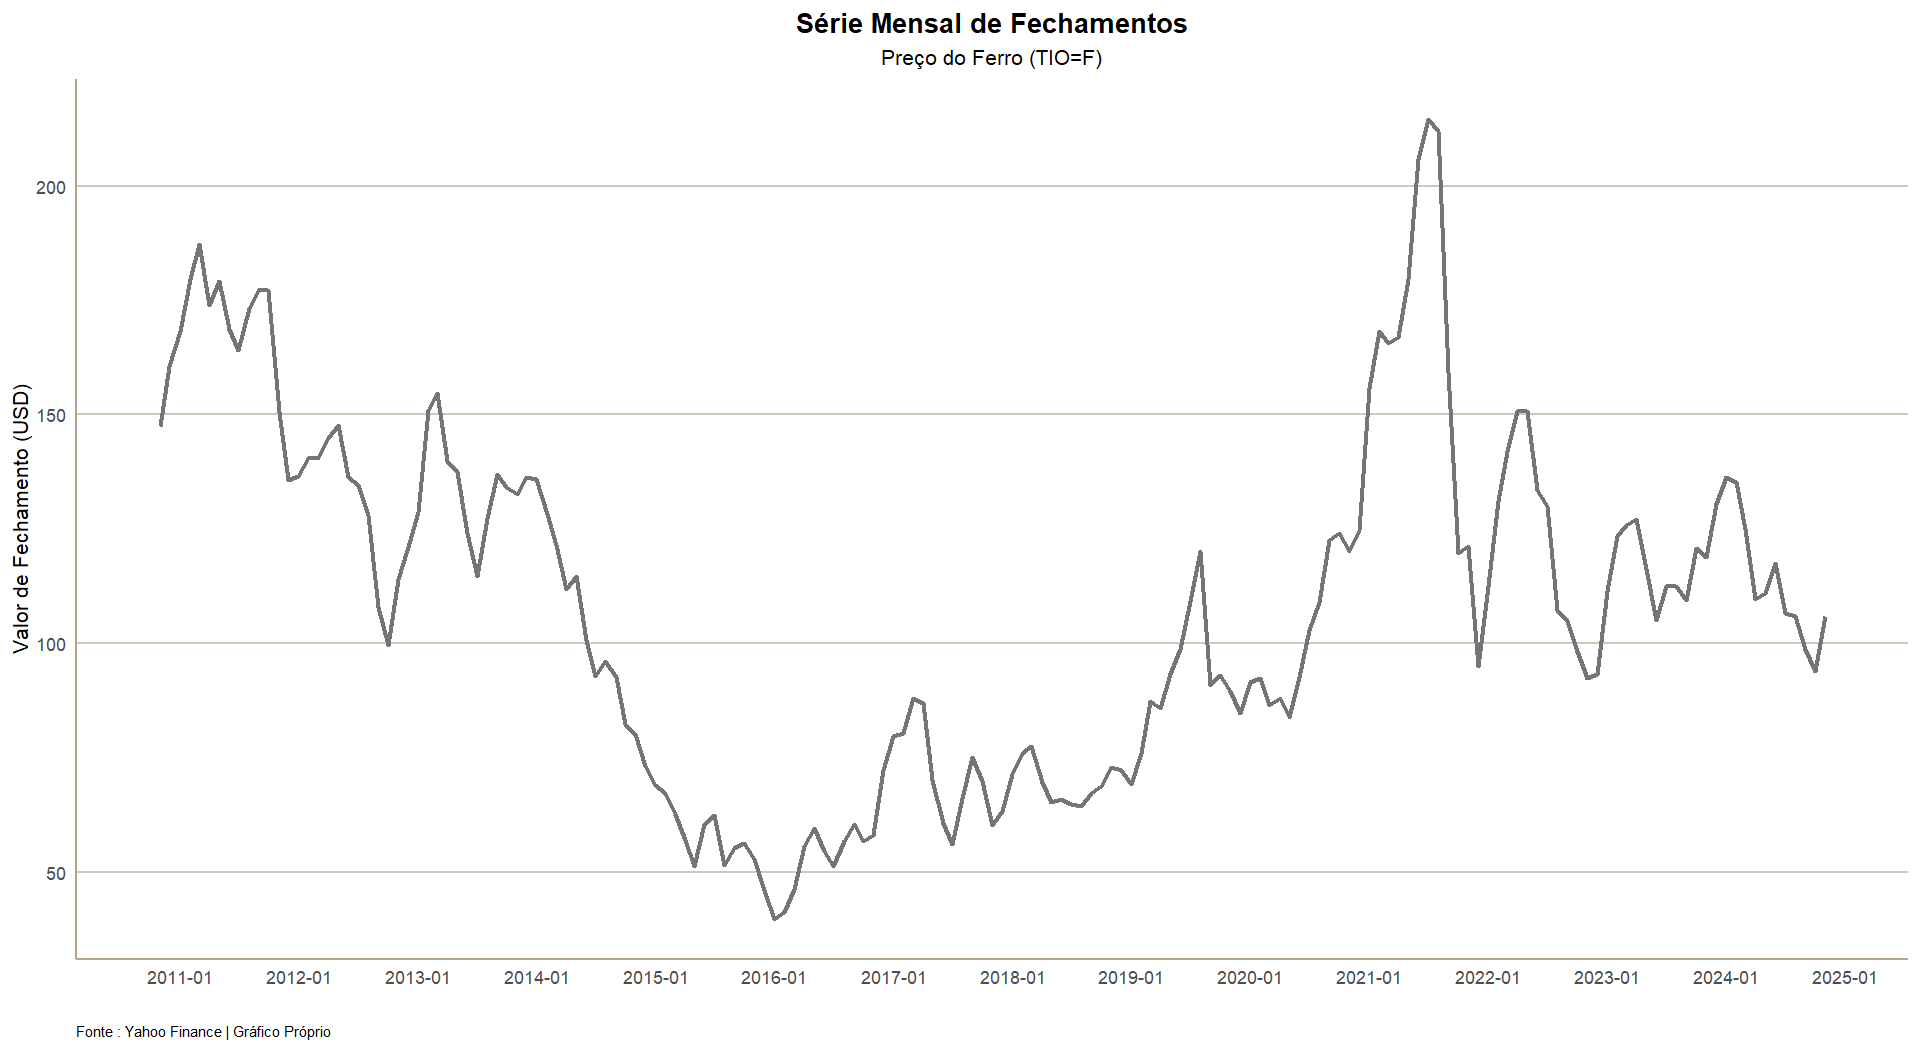
\includegraphics[width=1.0\textwidth]{APS 2/i1qA.png}
    \label{fig:i1qA}
    
    \footnotesize{Fonte: Elaborado pelos autores.}
    \end{figure}

\begin{figure}[H]
    \centering
    \caption{Série Mensal de Fechamentos do Preço do Ferro (TIO=F) - Últimos Dois Anos} 
    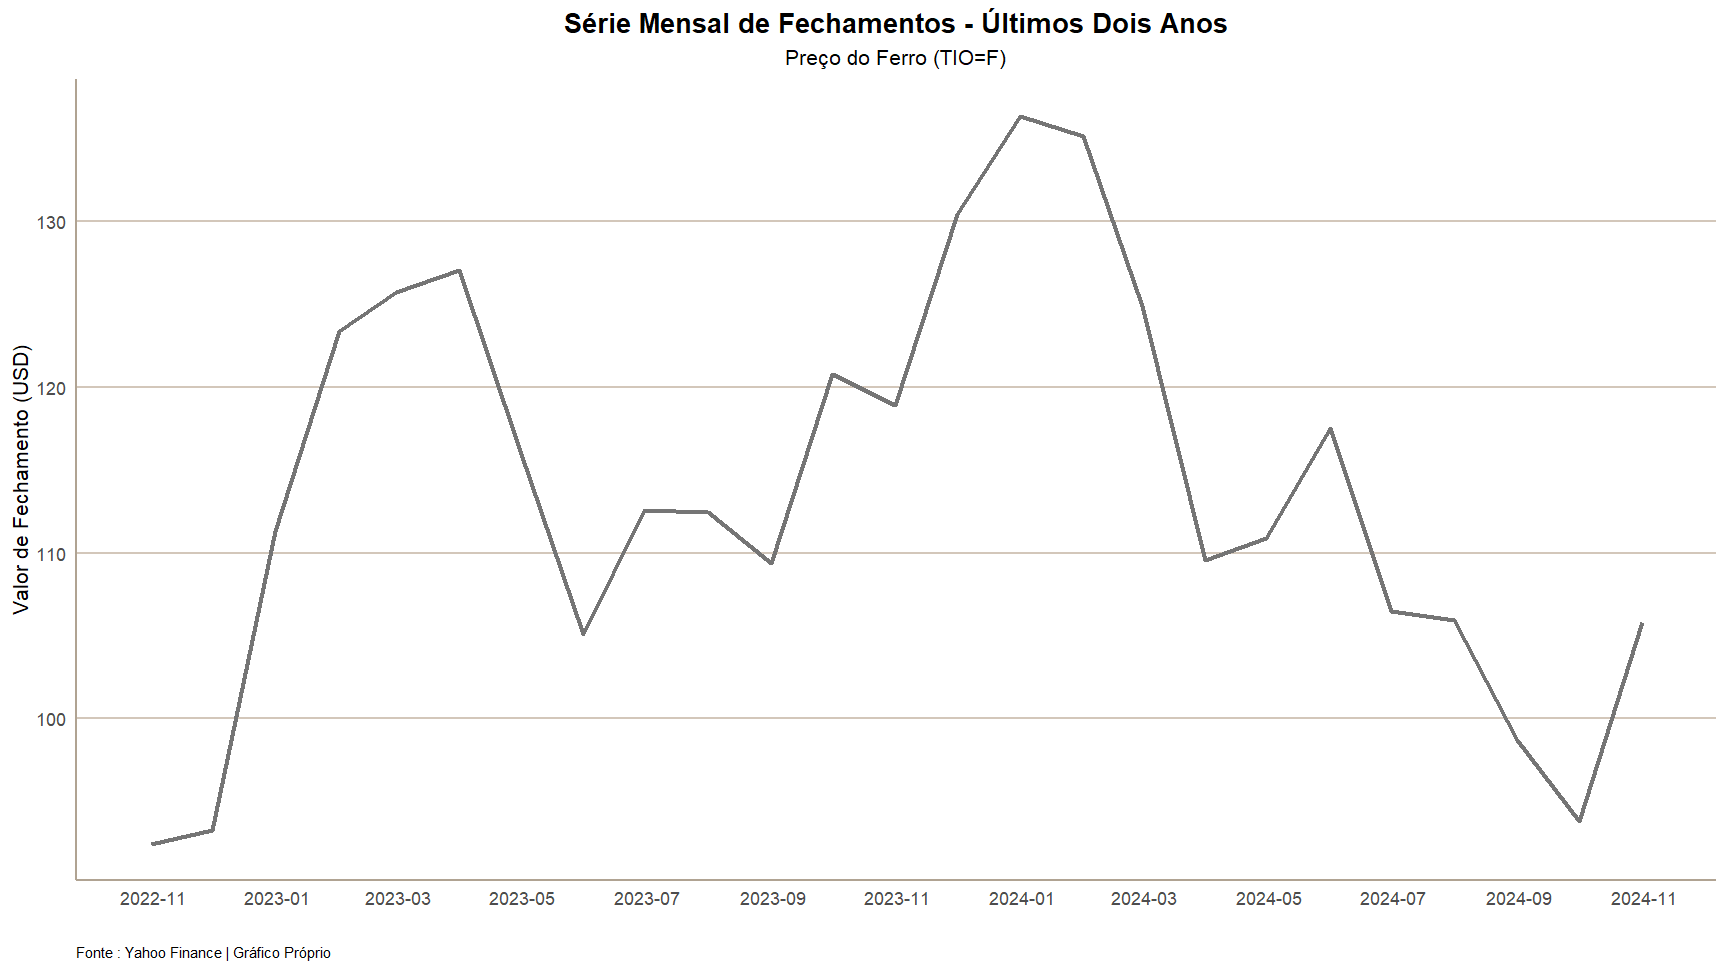
\includegraphics[width=1.0\textwidth]{APS 2/i2qA.png}
    \label{fig:i2qA}
    
    \footnotesize{Fonte: Elaborado pelos autores.}
    \end{figure}    
Com base nos dois gráficos da série mensal de fechamentos do preço do ferro, pode-se observar que o preço do minério de ferro tem se mostrado muito volátil ao longo dos últimos dois anos. 
Ao observar o gráfico \ref{fig:i1qA}, é notável que o preço do minério de ferro estava elevado, que pode ser atribuído ao aumento da demanda global pela commodity, especialmente, pela China para atender os seus projetos de infraestrutura. Após isso, houve uma queda acentuada do preço até 2015, caindo par um valor menor do que USD 50,00, sendo afetado pela desaceleração do crescimento econômico da China, diminuindo a demanda por minério de ferro, acarretando na diminuição do preço do ferro. 
Entre 2016 e 2019, o gráfico indica estabilidade do preço em relação aos outros períodos, seguida pelo aumento do preço em 2020 e 2021 que foi impulsionado pela recuperação econômica global após o impacto inicial da pandemia de COVID-19, especialmente com a retomada da demanda de infraestrutura e construção na China. 

A combinação de interrupções na cadeia de suprimentos e medidas de estímulo econômico global também contribuíram para o aumento nos preços das commodities, incluindo o minério de ferro. Após esse pico, observa-se uma correção acentuada no preço em 2022, com uma queda significativa. Essa queda pode ter sido influenciada pela desaceleração econômica global, pressões inflacionárias e políticas de controle de emissões que impactaram a produção de aço, especialmente na China.

A partir de janeiro de 2023, houve, novamente, um aumento acentuado, alcançando USD 130 em abril de 2023. Em 2024, houve uma queda acentuada pela diminuição na demanda global, somada a fatores como a guerra na Ucrânia e o aumento nos custos de energia, impactou os mercados de commodities e contribuiu para essa queda. 

\section*{\textbf{Questão B}}
\addcontentsline{toc}{section}{Questão B}

\begin{figure}[H]
    \centering
    \caption{Série Mensal de Fechamentos da Vale (VALE)} 
    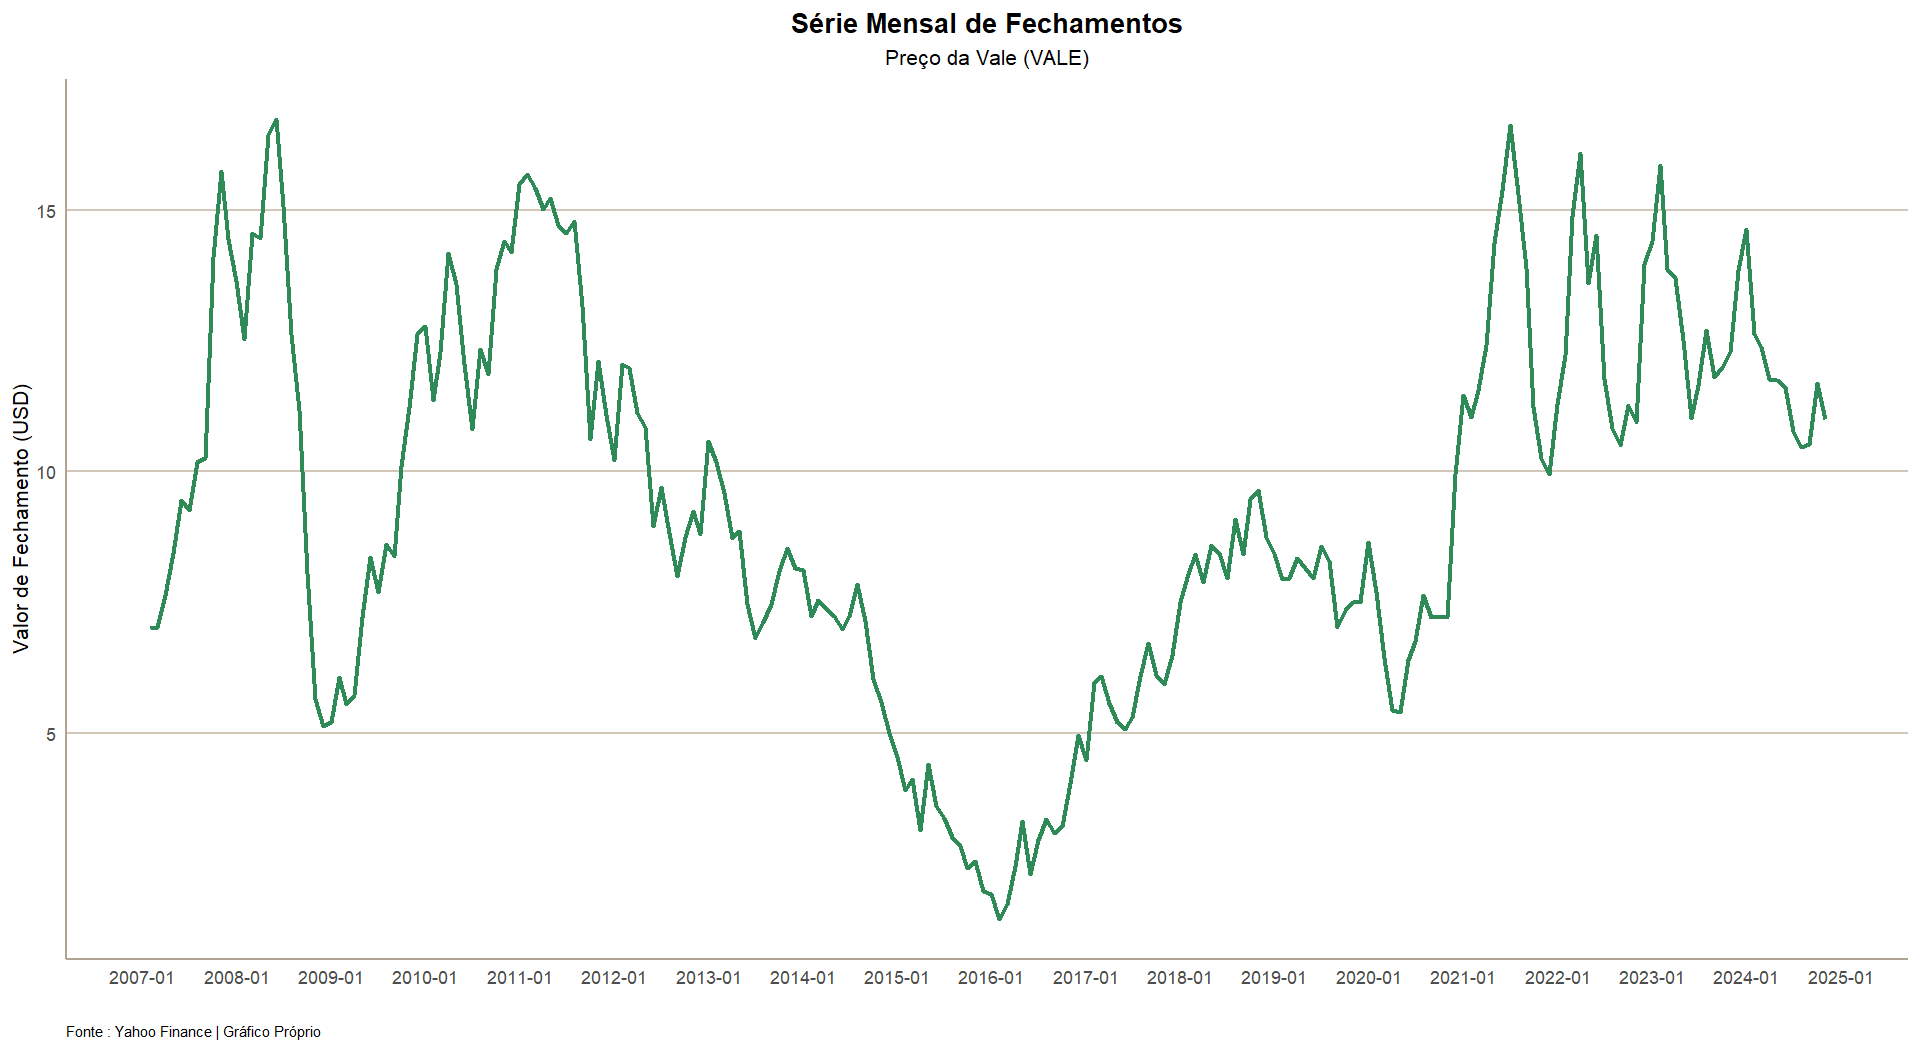
\includegraphics[width=1.0\textwidth]{APS 2/i1qB.png}
    \label{fig:i1qB}
    
    \footnotesize{Fonte: Elaborado pelos autores.}
    \end{figure}
O gráfico apresenta um primeiro pico significativo em 2008, com o preço das ações da Vale ultrapassando USD 15. Esse aumento pode estar relacionado ao forte crescimento das commodities e ao boom econômico pré-crise financeira global. A demanda por minério de ferro, produto principal da Vale, estava em alta, principalmente devido ao crescimento da China. Após o pico de 2008, há uma queda acentuada, com o preço das ações caindo rapidamente durante a crise financeira global de 2008-2009. A recessão global reduziu a demanda por commodities, impactando negativamente o preço das ações de empresas ligadas ao setor de mineração e materiais.

A partir de 2009, o gráfico mostra uma recuperação rápida e significativa, com o preço das ações da Vale retornando para níveis próximos de USD 15 em 2011. Este período coincide com a recuperação econômica global e com a retomada da demanda por commodities, principalmente pela China, que voltou a investir em infraestrutura. Entre 2011 e 2016, o preço das ações da Vale sofreu uma queda prolongada e contínua, atingindo seu ponto mais baixo em torno de USD 3 em 2016. Isso foi causado por uma combinação de fatores, como o excesso de oferta de minério de ferro no mercado global, a desaceleração do crescimento econômico da China e o colapso nos preços de várias commodities. Além disso, a tragédia de Mariana em 2015, que envolveu o rompimento de uma barragem da Samarco, também pode ter impactado negativamente o preço das ações, devido à perda de produção e à repercussão negativa no mercado.
A partir de 2016, o gráfico mostra uma nova recuperação do preço das ações da Vale, com uma tendência de alta que culmina em um novo pico em 2021, com o preço atingindo novamente valores acima de USD 15. Essa recuperação foi impulsionada pela retomada da demanda por minério de ferro e pela reorganização das operações da Vale após a tragédia.

A partir de 2021, o gráfico mostra um comportamento mais volátil, com altos e baixos acentuados, refletindo as incertezas econômicas globais pós-pandemia. O pico em 2021 coincide com a alta demanda por minério de ferro após a reabertura das economias e a recuperação pós-pandemia, enquanto as quedas subsequentes podem ser explicadas pela desaceleração da economia chinesa, controle de produção de aço e fatores ambientais. Entre 2022 e 2024, observa-se um comportamento instável, com quedas seguidas de pequenas recuperações, possivelmente refletindo as flutuações na demanda global por minério de ferro e as incertezas nos mercados financeiros.

\section*{\textbf{Questão C}}
\addcontentsline{toc}{section}{Questão C}

\begin{figure}[H]
    \centering
    \caption{Série Mensal dos Fechamentos} 
    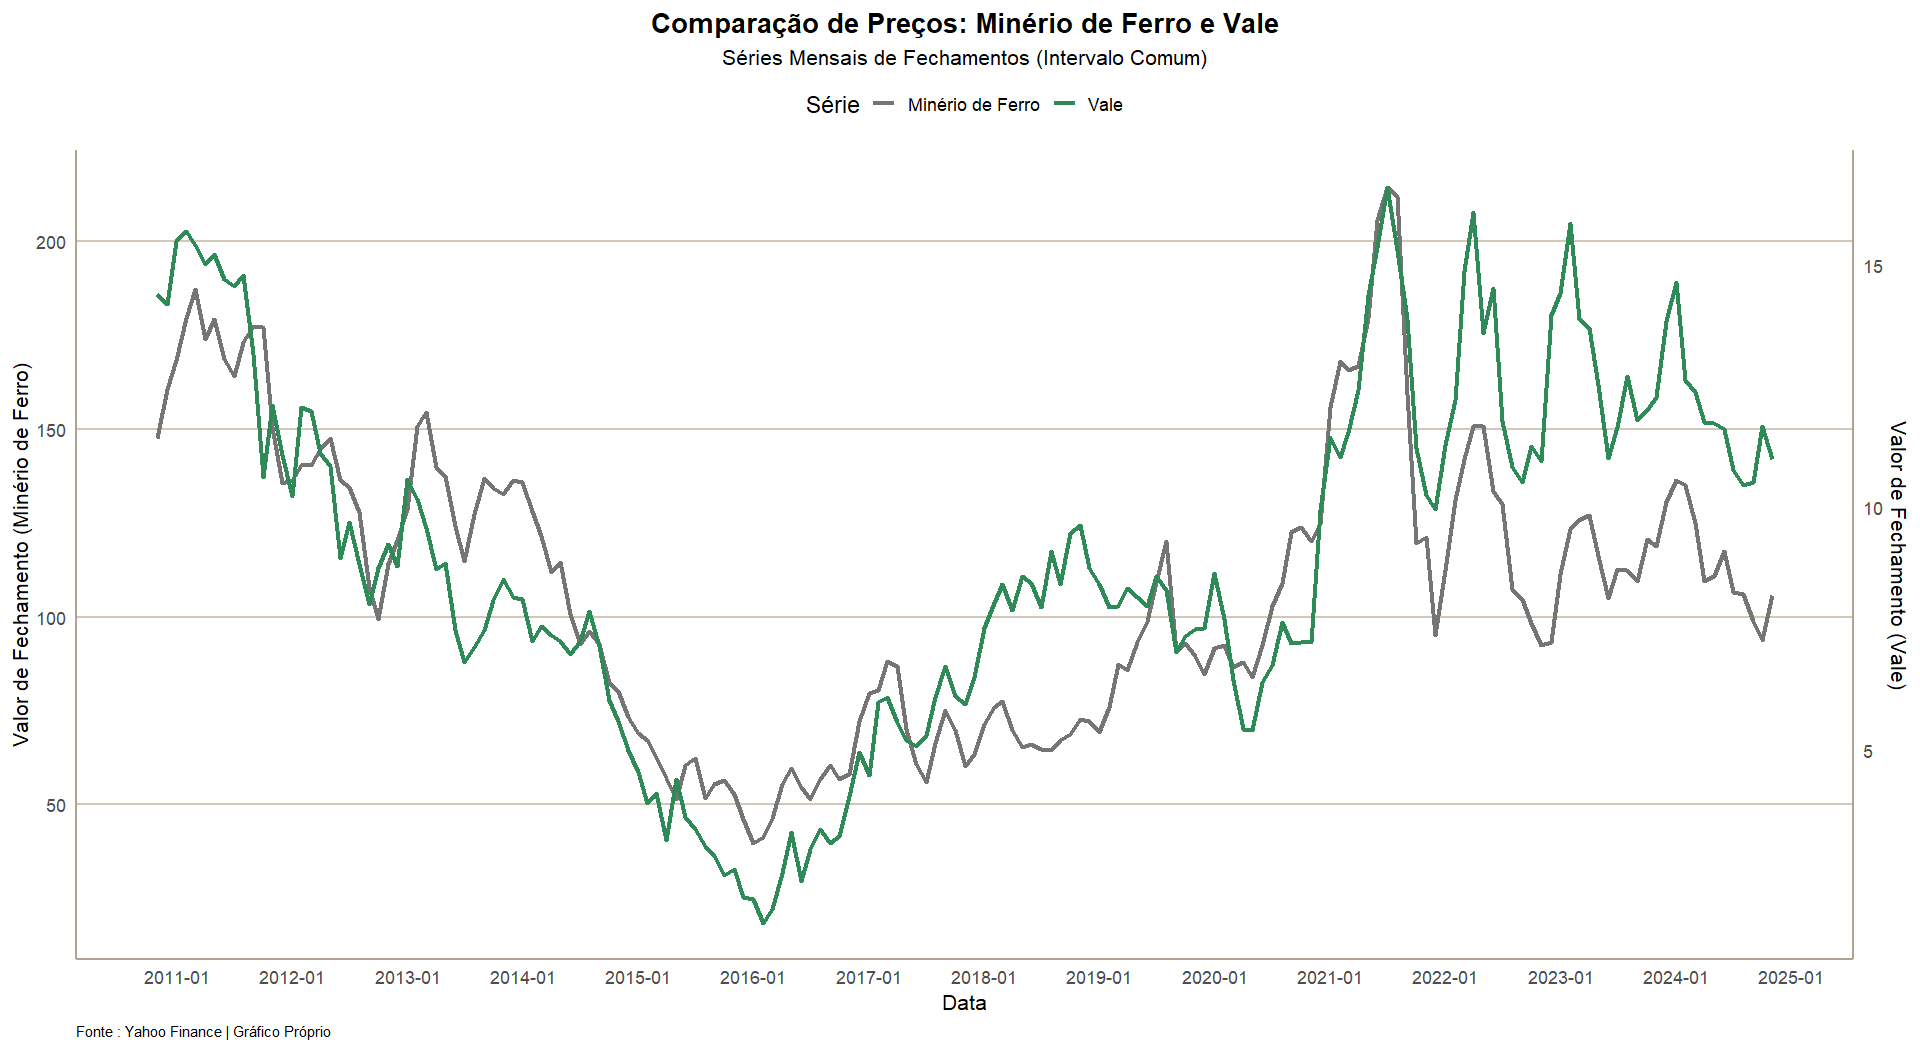
\includegraphics[width=1.0\textwidth]{APS 2/i1qC.png}
    \label{fig:i1qC}
    
    \footnotesize{Fonte: Elaborado pelos autores.}
    \end{figure}
O gráfico acima mostra que o preço do minério de ferro e o preço das ações da Vale seguem uma correlação bastante forte ao longo do período analisado. Isso é evidenciado nos momentos de alta e baixa da commodity como o que ocorreu entre 2011 e 2015. Nesse período, a queda no preço do minério de ferro, de mais de USD 200 para menos de USD 50, foi acompanhada pela queda significativa nas ações da Vale de mais de USD 15 para menos de USD 5. Esse movimento reflete a dependência da Vale na extração e venda de minério de ferro, como foi o caso durante a desaceleração do crescimento econômico da China e o excesso de oferta global, o desempenho financeiro da Vale é impactado negativamente, e suas ações perdem valor no mercado.

A partir de 2016, ambas as séries mostram uma recuperação, com o preço do minério de ferro subindo gradualmente e as ações da Vale acompanhando essa tendência. Essa recuperação foi impulsionada pela retomada da demanda global, especialmente pela China, e pela estabilização do mercado de commodities, após um período de queda prolongada. A correlação entre as duas séries atinge um ponto máximo em 2021, quando o preço do minério de ferro ultrapassa USD 200, refletindo o aumento abrupto da demanda global de matérias-primas para infraestrutura e construção, após a reabertura das economias durante a recuperação da pandemia de COVID-19. As ações da Vale também atingiram um pico nesse período, embora o aumento tenha sido menos acentuado em comparação ao minério de ferro, possivelmente devido a preocupações operacionais e riscos de longo prazo relacionados à sustentabilidade e à gestão de recursos naturais.

No período de 2022 a 2024, ambas as séries exibem comportamento volátil, com quedas significativas seguidas de pequenas recuperações. A principal explicação para essa volatilidade está na desaceleração econômica global, a redução na demanda por minério de ferro e as incertezas relacionadas à economia chinesa, maior consumidora mundial de aço. A volatilidade no preço do minério de ferro é rapidamente transmitida ao valor das ações da Vale, refletindo como a receita e o desempenho da empresa são diretamente afetados pelo mercado global de commodities.

Embora o comportamento geral das duas séries seja fortemente correlacionado, há períodos de divergência onde o preço das ações da Vale e o preço do minério de ferro não se movem em sincronia. Isso ocorre principalmente devido a fatores específicos da empresa. Um exemplo notável é a tragédia de Mariana em 2015, que resultou em uma forte queda nas ações da Vale, enquanto o preço do minério de ferro já vinha em queda, mas não tão abrupta. Esses eventos mostram que, além da relação com a commodity, o preço das ações da Vale também é sensível a eventos internos, como desastres ambientais, desafios operacionais, e a gestão de crises.

\section*{\textbf{Questão D}}
\addcontentsline{toc}{section}{Questão D}

\begin{figure}[H]
    \centering
    \caption{Série Mensal dos Fechamentos em Logaritmo Natural} 
    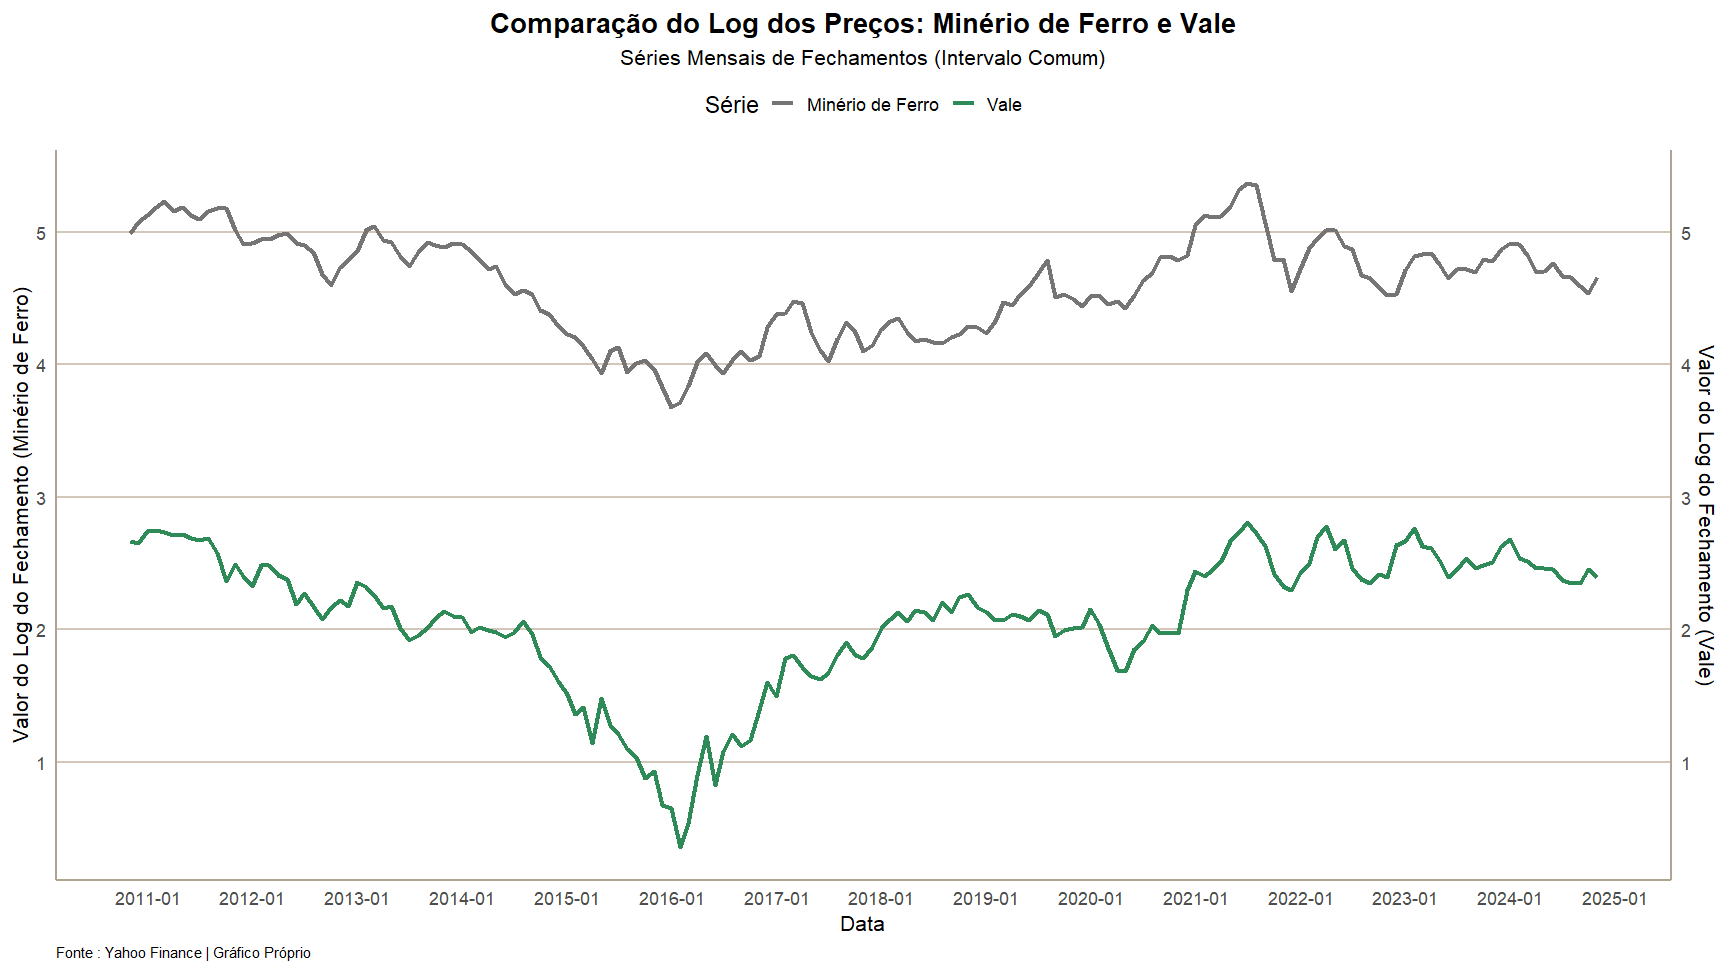
\includegraphics[width=1.0\textwidth]{APS 2/i1qD.png}
    \label{fig:i1qD}
    
    \footnotesize{Fonte: Elaborado pelos autores.}
    \end{figure}

O gráfico da série mensal dos fechamentos em logaritmo natural nos fornece uma visão mais clara e ajustada das flutuações relativas entre as duas séries. A aplicação do logaritmo natural permite suavizar grandes variações, tornando mais evidente a relação entre os dois ativos, que já foi analisada anteriormente com os preços absolutos. Essa transformação ajuda a destacar a correlação entre as variações de preço, além de permitir uma melhor comparação do comportamento percentual ao longo do tempo.

Ao longo do período analisado, é evidente que há uma forte correlação entre o comportamento do preço do minério de ferro e das ações da Vale. A Vale, sendo uma das maiores mineradoras de minério de ferro do mundo, depende fortemente da demanda e dos preços dessa commodity. Quando o preço do minério de ferro sobe ou desce, o valor das ações da Vale tende a seguir a mesma direção.

Durante o período de 2011 a 2015, ambas as séries mostram uma queda acentuada. O logaritmo do preço do minério de ferro, assim como o das ações da Vale, diminui significativamente, o que reflete o impacto direto que a queda da commodity tem sobre o valor de mercado da empresa. Esse período foi marcado pela desaceleração da economia chinesa e pelo excesso de oferta de minério de ferro no mercado global, o que resultou em uma queda acentuada nos preços.
A ação da Vale espelha esse movimento porque suas receitas são altamente dependentes do minério de ferro. Assim, uma queda no preço da commodity pressiona os lucros da empresa e, consequentemente, o valor de suas ações.

Já entre 2016 e 2021, ambas as séries mostram uma recuperação notável. O logaritmo natural do preço do minério de ferro começa a subir, impulsionado pela retomada da demanda global, principalmente pela China. As ações da Vale também seguem essa tendência, com o logaritmo natural mostrando um movimento ascendente, embora com uma volatilidade um pouco menor.
Esse comportamento reafirma a relação direta entre os dois ativos: a Vale, ao aumentar suas receitas com a venda de minério de ferro a preços mais altos, ganha valor no mercado, e suas ações sobem em sintonia com o preço da commodity.

Em 2021 representa um ponto alto para ambas as séries, onde o preço do minério de ferro atinge seu pico, e as ações da Vale também experimentam um aumento expressivo. Esse aumento foi impulsionado pela recuperação econômica global após o auge da pandemia de COVID-19, quando a demanda por aço, e consequentemente por minério de ferro, aumentou drasticamente, especialmente na China.
Após o pico em 2021, o logaritmo natural de ambas as séries começa a mostrar sinais de volatilidade, com uma leve tendência de queda, mas também com algumas recuperações. Essa volatilidade reflete as incertezas econômicas e geopolíticas globais, incluindo a desaceleração da economia chinesa e as políticas ambientais que afetam a produção de aço.

Embora ambas as séries sigam um padrão geral semelhante, existem algumas diferenças na magnitude das variações. As ações da Vale tendem a exibir uma volatilidade um pouco menor em comparação com o preço do minério de ferro, especialmente em períodos de forte queda ou alta. Isso pode ser explicado pelo fato de que, além do minério de ferro, a Vale também diversifica suas operações com outros minerais e atividades, o que ajuda a amortecer as variações extremas de preço.
No entanto, apesar dessa diferença, a direção dos movimentos das duas séries permanece altamente correlacionada, reforçando a forte dependência da Vale em relação ao minério de ferro. Quando o preço do minério de ferro sobe, as ações da Vale tendem a subir, e quando o preço cai, as ações da empresa seguem a mesma direção, embora de maneira menos acentuada.

\section*{\textbf{Questão E}}
\addcontentsline{toc}{section}{Questão E}

Nesse item, os resultados de 3 configurações do Teste ADF aplicados à série logarítmica dos preços dos minérios de ferro serão discutidos. Sendo que as hipóteses do teste serão dadas por:

\[
\left\{
\begin{array}{ll}
    \text{Hipótese Nula } H_0: & \gamma = 0 \ (\text{A série tem uma raiz unitária}) \\
    \text{Hipótese Alternativa } H_a: & \gamma \leqslant 0 \ (\text{A série não tem raiz unitária})
\end{array}
\right.
\]


\begin{equation}
    \Delta Log(pf)_t = \alpha + \beta t + \gamma Log(pf)_{t-1} + \delta \Delta Log(pf)_{t-1} + a_t \ \ ; \ \ a_t \sim RB(0, \sigma_a^2)   
    \label{eq:taltallpf}
\end{equation}

\begin{table}[H] 
  \centering 
  \caption{Resultados do Teste ADF do Log dos Preços do Ferro (TIO=F) com Tendência, Intercepto e Defasagens} 
  \label{tab:adftotalferro} 
  \renewcommand{\arraystretch}{0.9} % Reduz o espaçamento entre as linhas
  \resizebox{0.9\textwidth}{!}{ % Reduz a largura da tabela para 90% da largura do texto
    \footnotesize % Usa uma fonte menor
    \begin{tabular}{@{\extracolsep{5pt}}lccc} 
      \\[-1.8ex]\hline 
      \hline \\[-1.8ex] 
      & Estimate & Std. Error & t value \\ 
      \hline \\[-1.8ex] 
      $\alpha$ \textbf{(Intercepto)} & $0.2353$ & $0.0940$ & $2.503^{*}$ \\ 
      $\gamma$ \textbf{(Coef UR)} & $-0.0556$ & $0.0206$ & $-2.694^{**}$ \\ 
      $\beta$ \textbf{(Coef Trend)} & $0.0002$ & $0.0002$ & $1.156$ \\ 
      $\delta$ \textbf{(Coef Lag)} & $0.2804$ & $0.0767$ & $3.657^{***}$ \\ 
      \hline \\[-1.8ex] 
      Erro padrão residual & \multicolumn{3}{c}{$0.09258$ \textit{(df = 154)}} \\ 
      R-quadrado múltiplo & \multicolumn{3}{c}{$0.1147$} \\ 
      R-quadrado ajustado & \multicolumn{3}{c}{$0.09743$} \\ 
      Estatística-F & \multicolumn{3}{c}{$6.65$ \textit{(df = 3; 154)}, p-value: $0.0002981$} \\ 
      Valor do Teste & \multicolumn{3}{c}{$-2.6936$, $2.6708$, $3.9597$} \\ 
      \hline 
      Critical values for test statistics & \multicolumn{3}{c}{} \\ 
      1pct ($\gamma$)  & \multicolumn{3}{c}{$-3.99$} \\ 
      5pct ($\gamma$)  & \multicolumn{3}{c}{$-3.43$} \\ 
      10pct ($\gamma$) & \multicolumn{3}{c}{$-3.13$} \\ 
      1pct ($\alpha$)  & \multicolumn{3}{c}{$6.22$} \\ 
      5pct ($\alpha$)  & \multicolumn{3}{c}{$4.75$} \\ 
      10pct ($\alpha$) & \multicolumn{3}{c}{$4.07$} \\ 
      1pct ($\beta$)   & \multicolumn{3}{c}{$8.43$} \\ 
      5pct ($\beta$)   & \multicolumn{3}{c}{$6.49$} \\ 
      10pct ($\beta$)  & \multicolumn{3}{c}{$5.47$} \\ 
      \hline 
      \hline \\[-1.8ex] 
      \textit{Note:} & \multicolumn{3}{r}{$^{*}$Significant at 5\% level, $^{**}$Significant at 1\% level, $^{***}$Significant at 0.1\% level} \\ 
    \end{tabular} 
  }
\end{table}

O primeiro modelo (equação \ref{eq:taltallpf}) apresentado inclui uma tendência linear, um intercepto e defasagens, que ajustam as flutuações passadas da série.

O coeficiente do intercepto ($\alpha$ = 0,2253) indica o valor médio esperado do log dos preços de ferro, quando todos os outros termos são iguais a 0, ou seja, na ausência de uma tendência temporal e de defasagens.

O valor estimado para o coeficiente da raiz unitária ($\gamma$) é de -0,0556, o que sugere a presença de raiz unitária na série, pois o valor é negativo. No qual o valor da estatística $\tau$ de -2,694 está fora de todas as regiões críticas seja com níveis de confiança de 1\%, 5\% ou 10\%, trazendo indícios de não rejeição da hipótese nula.

O coeficiente de tendência ($\beta$ = 0,0002) indica uma possível tendência positiva, embora muito fraca; no entanto, seu valor reduzido sugere que essa tendência não é estatisticamente significativa para influenciar o comportamento da série. 

O coeficiente de defasagem ($\delta = 0,2804$) revela uma dependência em relação às variações passadas do preço do minério de ferro, o que justifica a inclusão de defasagens no modelo para assegurar que o erro seja um ruído branco.



\begin{equation}
    \Delta Log(pf)_t = \alpha + \gamma Log(pf)_{t-1} + \delta \Delta Log(pf)_{t-1} + a_t \ \ ; \ \ a_t \sim RB(0, \sigma_a^2)   
    \label{eq:talinterceptopf}
\end{equation}

\begin{table}[H] \centering 
  \caption{Resultados do Teste ADF do Log dos Preços do Ferro (TIO=F) sem Tendência, com Intercepto e com Defasagens} 
  \renewcommand{\arraystretch}{0.9} % Reduz o espaçamento entre as linhas
  \resizebox{0.9\textwidth}{!}{ % Reduz a largura da tabela para 90% da largura do texto
    \footnotesize % Usa uma fonte menor
  \begin{tabular}{@{\extracolsep{5pt}}lccc} 
  \\[-1.8ex]\hline 
  \hline \\[-1.8ex] 
  & Estimate & Std. Error & t value \\ 
  \hline \\[-1.8ex] 
  $\alpha$ (\textbf{Intercepto}) & $0.2381$ & $0.0941$ & $2.531^{*}$ \\ 
  $\gamma$ (\textbf{Coef UR}) & $-0.0525$ & $0.0205$ & $-2.563^{*}$ \\ 
  $\delta$ (\textbf{Coef Lag} )& $0.2847$ & $0.0767$ & $3.712^{***}$ \\ 
  \hline \\[-1.8ex] 
  Erro padrão residual & \multicolumn{3}{c}{$0.09268$ \textit{(df = 155)}} \\ 
  R-quadrado múltiplo & \multicolumn{3}{c}{$0.107$} \\ 
  R-quadrado ajustado & \multicolumn{3}{c}{$0.09547$} \\ 
  Estatística-F & \multicolumn{3}{c}{$9.286$ \textit{(df = 2; 155)}, p-value: $0.0001553$} \\ 
  Valor do Teste & \multicolumn{3}{c}{$-2.5628$, $3.3304$} \\ 
  \hline 
  Critical values for test statistics & \multicolumn{3}{c}{} \\ 
  1pct ($\gamma$) & \multicolumn{3}{c}{$-3.46$} \\ 
  5pct ($\gamma$) & \multicolumn{3}{c}{$-2.88$} \\ 
  10pct ($\gamma$) & \multicolumn{3}{c}{$-2.57$} \\ 
  1pct ($\alpha$) & \multicolumn{3}{c}{$6.52$} \\ 
  5pct ($\alpha$) & \multicolumn{3}{c}{$4.63$} \\ 
  10pct ($\alpha$) & \multicolumn{3}{c}{$3.81$} \\ 
  \hline 
  \hline \\[-1.8ex] 
  \textit{Note:} & \multicolumn{3}{r}{$^{*}$Significant at 5\% level, $^{**}$Significant at 1\% level, $^{***}$Significant at 0.1\% level} \\ 
  \end{tabular} 
  }
  \label{tab:adfinterceptoferro}
\end{table}

O segundo modelo (equação \ref{eq:talinterceptopf}) apresentado inclui um intercepto e defasagens, que ajustam as flutuações passadas da série.

O valor estimado para o coeficiente da raiz unitária ($\gamma$) é de -0,0525 com o valor da estatística $\tau$ de -2,563, o que sugere a presença de raiz unitária na série (para 1\% e 5\% de significância). O coeficiente de intercepto ($\alpha = 0,2381$) indica um possível intercepto, sua estatística apresenta um valor estatisticamente significante. O coeficiente de defasagem ($\delta = 0,2847$) revela uma dependência em relação às variações passadas do preço do minério de ferro, o que justifica a inclusão de defasagens no modelo para assegurar que o erro seja um ruído branco.

\begin{equation}
    \Delta Log(pf)_t = \gamma Log(pf)_{t-1} + \delta \Delta Log(pf)_{t-1} + a_t \ \ ; \ \ a_t \sim RB(0, \sigma_a^2)   
    \label{eq:tallpf}
\end{equation}

\begin{table}[H] \centering 
  \caption{Resultados do Teste ADF do Log dos Preços do Ferro (TIO=F) Apenas com Defasagens} 
  \renewcommand{\arraystretch}{0.9} % Reduz o espaçamento entre as linhas
  \resizebox{0.9\textwidth}{!}{ % Reduz a largura da tabela para 90% da largura do texto
    \footnotesize % Usa uma fonte menor
  \begin{tabular}{@{\extracolsep{5pt}}lccc} 
  \\[-1.8ex]\hline 
  \hline \\[-1.8ex] 
  & Estimate & Std. Error & t value \\ 
  \hline \\[-1.8ex] 
  $\gamma$ (\textbf{Coef UR})& $-0.0008$ & $0.0016$ & $-0.496$ \\ 
  $\delta$ (\textbf{Coef Lag}) & $0.2640$ & $0.0776$ & $3.403^{***}$ \\ 
  \hline \\[-1.8ex] 
  Erro padrão residual & \multicolumn{3}{c}{$0.09428$ \textit{(df = 156)}} \\ 
  R-quadrado múltiplo & \multicolumn{3}{c}{$0.07114$} \\ 
  R-quadrado ajustado & \multicolumn{3}{c}{$0.05923$} \\ 
  Estatística-F & \multicolumn{3}{c}{$5.974$ \textit{(df = 2; 156)}, p-value: $0.003163$} \\ 
  Valor do Teste & \multicolumn{3}{c}{$-0.4961$} \\ 
  \hline 
  Critical values for test statistics & \multicolumn{3}{c}{} \\ 
  1pct ($\gamma$) & \multicolumn{3}{c}{$-2.58$} \\ 
  5pct ($\gamma$) & \multicolumn{3}{c}{$-1.95$} \\ 
  10pct ($\gamma$) & \multicolumn{3}{c}{$-1.62$} \\ 
  \hline 
  \hline \\[-1.8ex] 
  \textit{Note:} & \multicolumn{3}{r}{$^{*}$Significant at 5\% level, $^{**}$Significant at 1\% level, $^{***}$Significant at 0.1\% level} \\ 
  \end{tabular} 
 }
 \label{tab:adfferro}
\end{table}

O terceiro modelo (equação \ref{eq:tallpf}) apresentado inclui um intercepto e defasagens, que ajustam as flutuações passadas da série.

O valor estimado para o coeficiente da raiz unitária ($\gamma$) é de -0,0008 o que sugere a presença de raiz unitária na série, já que a estatística (-0,496) se encontra fora do intervalo de confiança. O coeficiente de defasagem ($\delta = 0,2847$) revela uma dependência em relação às variações passadas do preço do minério de ferro, o que justifica a inclusão de defasagens no modelo para assegurar que o erro seja um ruído branco.

Concluímos, com base nos três testes, que o logaritmo do preço do ferro segue um processo estocástico, devido à presença de raiz unitária. No entanto, fundamentados na teoria financeira, como estamos modelando o preço de um ativo cujo valor inicial não é zero, devemos optar pelo segundo modelo, que inclui um intercepto.

\section*{\textbf{Questão F}}
\addcontentsline{toc}{section}{Questão F}

\[
\left\{
\begin{array}{ll}
    \text{Hipótese Nula } H_0: & \gamma = 0 \ (\text{A série tem uma raiz unitária}) \\
    \text{Hipótese Alternativa } H_a: & \gamma \leqslant 0 \ (\text{A série não tem raiz unitária})
\end{array}
\right.
\]

\begin{equation}
    \Delta Log(pv)_t = \alpha + \beta t + \gamma Log(pv)_{t-1} + \delta \Delta Log(pv)_{t-1} + a_t \ \ ; \ \ a_t \sim RB(0, \sigma_a^2)   
    \label{eq:taltallpv}
\end{equation}

% Resultados do Teste ADF com Tendência, Intercepto e Defasagens
\begin{table}[H] \centering 
  \caption{Resultados do Teste ADF do Log dos Preço da Vale (VALE)  com Tendência, Intercepto e Defasagens} 
  \renewcommand{\arraystretch}{0.9} % Reduz o espaçamento entre as linhas
  \resizebox{0.9\textwidth}{!}{ % Reduz a largura da tabela para 90% da largura do texto
    \footnotesize % Usa uma fonte menor
  \begin{tabular}{@{\extracolsep{5pt}}lccc} 
  \\[-1.8ex]\hline 
  \hline \\[-1.8ex] 
  & Estimate & Std. Error & t value \\ 
  \hline \\[-1.8ex] 
  $\alpha$ (\textbf{Intercepto}) & $0.0624$ & $0.0411$ & $1.518$ \\ 
  $\gamma$ (\textbf{Coef UR}) & $-0.0362$ & $0.0175$ & $-2.071^{*}$ \\ 
  $\beta$ (\textbf{Coef Trend}) & $0.0001$ & $0.0001$ & $0.810$ \\ 
  $\delta$ (\textbf{Coef Lag}) & $0.0880$ & $0.0704$ & $1.250$ \\ 
  \hline \\[-1.8ex] 
  Erro padrão residual & \multicolumn{3}{c}{$0.123$ \textit{(df = 199)}} \\ 
  R-quadrado múltiplo & \multicolumn{3}{c}{$0.02924$} \\ 
  R-quadrado ajustado & \multicolumn{3}{c}{$0.01461$} \\ 
  Estatística-F & \multicolumn{3}{c}{$1.998$ \textit{(df = 3; 199)}, p-value: $0.1155$} \\ 
  Valor do Teste & \multicolumn{3}{c}{$-2.0706$, $1.6167$, $2.4148$} \\ 
  \hline 
  Critical values for test statistics & \multicolumn{3}{c}{} \\ 
  1pct ($\gamma$) & \multicolumn{3}{c}{$-3.99$} \\ 
  5pct ($\gamma$) & \multicolumn{3}{c}{$-3.43$} \\ 
  10pct ($\gamma$) & \multicolumn{3}{c}{$-3.13$} \\ 
  1pct ($\alpha$) & \multicolumn{3}{c}{$6.22$} \\ 
  5pct ($\alpha$) & \multicolumn{3}{c}{$4.75$} \\ 
  10pct ($\alpha$) & \multicolumn{3}{c}{$4.07$} \\ 
  1pct ($\beta$) & \multicolumn{3}{c}{$8.43$} \\ 
  5pct ($\beta$) & \multicolumn{3}{c}{$6.49$} \\ 
  10pct ($\beta$) & \multicolumn{3}{c}{$5.47$} \\ 
  \hline 
  \hline \\[-1.8ex] 
  \textit{Note:} & \multicolumn{3}{r}{$^{*}$Significant at 5\% level, $^{**}$Significant at 1\% level, $^{***}$Significant at 0.1\% level} \\ 
  \end{tabular} 
  }
  \label{tab:adftotalvale}
\end{table}

O primeiro modelo (equação \ref{eq:taltallpv}) apresentado inclui uma tendência linear, um intercepto e defasagens, que ajustam as flutuações passadas da série.

O valor estimado para o coeficiente da raiz unitária ($\gamma$) é de 0,0624, o que sugere a presença de raiz unitária na série, já que a estatística (1,518) se encontra fora do intervalo de confiança. O coeficiente de tendência ($\beta = 0,0001$) indica uma possível tendência positiva, embora muito fraca; no entanto, seu valor reduzido sugere que essa tendência não é estatisticamente significativa para influenciar o comportamento da série. O coeficiente de defasagem ($\delta = 1.250$) revela uma dependência em relação às variações passadas do preço da vale, o que justifica a inclusão de defasagens no modelo para assegurar que o erro seja um ruído branco.

\begin{equation}
    \Delta Log(pv)_t = \alpha + \gamma Log(pv)_{t-1} + \delta \Delta Log(pv)_{t-1} + a_t \ \ ; \ \ a_t \sim RB(0, \sigma_a^2)   
    \label{eq:talinterceptopv}
\end{equation}

% Resultados do Teste ADF sem Tendência, com Intercepto e com Defasagens
\begin{table}[H] \centering 
  \caption{Resultados do Teste ADF do Log dos Preço da Vale (VALE) sem Tendência, com Intercepto e com Defasagens} 
  \renewcommand{\arraystretch}{0.9} % Reduz o espaçamento entre as linhas
  \resizebox{0.9\textwidth}{!}{ % Reduz a largura da tabela para 90% da largura do texto
    \footnotesize % Usa uma fonte menor
  \begin{tabular}{@{\extracolsep{5pt}}lccc} 
  \\[-1.8ex]\hline 
  \hline \\[-1.8ex] 
  & Estimate & Std. Error & t value \\ 
  \hline \\[-1.8ex] 
  $\alpha$ (\textbf{Intercepto}) & $0.0747$ & $0.0381$ & $1.959^{\cdot}$ \\ 
  $\gamma$ (\textbf{Coef UR}) & $-0.0357$ & $0.0175$ & $-2.045^{*}$ \\ 
  $\delta$ (\textbf{Coef Lag}) & $0.0915$ & $0.0702$ & $1.304$ \\ 
  \hline \\[-1.8ex] 
  Erro padrão residual & \multicolumn{3}{c}{$0.1229$ \textit{(df = 200)}} \\ 
  R-quadrado múltiplo & \multicolumn{3}{c}{$0.02604$} \\ 
  R-quadrado ajustado & \multicolumn{3}{c}{$0.0163$} \\ 
  Estatística-F & \multicolumn{3}{c}{$2.674$ \textit{(df = 2; 200)}, p-value: $0.07146$} \\ 
  Valor do Teste & \multicolumn{3}{c}{$-2.0447$, $2.1007$} \\ 
  \hline 
  Critical values for test statistics & \multicolumn{3}{c}{} \\ 
  1pct ($\gamma$) & \multicolumn{3}{c}{$-3.46$} \\ 
  5pct ($\gamma$) & \multicolumn{3}{c}{$-2.88$} \\ 
  10pct ($\gamma$) & \multicolumn{3}{c}{$-2.57$} \\ 
  1pct ($\alpha$) & \multicolumn{3}{c}{$6.52$} \\ 
  5pct ($\alpha$) & \multicolumn{3}{c}{$4.63$} \\ 
  10pct ($\alpha$) & \multicolumn{3}{c}{$3.81$} \\ 
  \hline 
  \hline \\[-1.8ex] 
  \textit{Note:} & \multicolumn{3}{r}{$^{*}$Significant at 5\% level, $^{**}$Significant at 1\% level, $^{***}$Significant at 0.1\% level} \\ 

  \end{tabular} 
  }
  \label{tab:adfinterceptovale}
\end{table}

O segundo modelo (equação \ref{eq:talinterceptopv}) apresentado inclui um intercepto e defasagens, que ajustam as flutuações passadas da série.

O valor estimado para o coeficiente da raiz unitária ($\gamma$) é de -0,0357, o que sugere a presença de raiz unitária na série, já que a estatística (-2,045)  se encontra fora do intervalo de confiança. O coeficiente de intercepto ($\alpha = 0,0747$) indica um possível intercepto, sua estatística apresenta um valor estatisticamente significante. O coeficiente de defasagem ($\delta = 0,0915$) revela uma dependência em relação às variações passadas do preço da vale, o que justifica a inclusão de defasagens no modelo para assegurar que o erro seja um ruído branco.

\begin{equation}
    \Delta Log(pv)_t = \gamma Log(pv)_{t-1} + \delta \Delta Log(pv)_{t-1} + a_t \ \ ; \ \ a_t \sim RB(0, \sigma_a^2)   
    \label{eq:tallpv}
\end{equation}

% Resultados do Teste ADF Apenas com Defasagens
\begin{table}[H] \centering 
  \caption{Resultados do Teste ADF do Log dos Preço da Vale (VALE) Apenas com Defasagens} 
  \renewcommand{\arraystretch}{0.9} % Reduz o espaçamento entre as linhas
  \resizebox{0.9\textwidth}{!}{ % Reduz a largura da tabela para 90% da largura do texto
    \footnotesize % Usa uma fonte menor
  \begin{tabular}{@{\extracolsep{5pt}}lccc} 
  \\[-1.8ex]\hline 
  \hline \\[-1.8ex] 
  & Estimate & Std. Error & t value \\ 
  \hline \\[-1.8ex]  
  $\gamma$ (\textbf{Coef UR}) & $-0.0024$ & $0.0040$ & $-0.598$ \\ 
  $\delta$ (\textbf{Coef Lag}) & $0.0760$ & $0.0702$ & $1.083$ \\ 
  \hline \\[-1.8ex] 
  Erro padrão residual & \multicolumn{3}{c}{$0.1237$ \textit{(df = 201)}} \\ 
  R-quadrado múltiplo & \multicolumn{3}{c}{$0.007464$} \\ 
  R-quadrado ajustado & \multicolumn{3}{c}{$-0.002412$} \\ 
  Estatística-F & \multicolumn{3}{c}{$0.7558$ \textit{(df = 2; 201)}, p-value: $0.471$} \\ 
  Valor do Teste & \multicolumn{3}{c}{$-0.5977$} \\ 
  \hline 
  Critical values for test statistics & \multicolumn{3}{c}{} \\ 
  1pct ($\gamma$) & \multicolumn{3}{c}{$-2.58$} \\ 
  5pct ($\gamma$) & \multicolumn{3}{c}{$-1.95$} \\ 
  10pct ($\gamma$) & \multicolumn{3}{c}{$-1.62$} \\ 
  \hline 
  \hline \\[-1.8ex]
  \textit{Note:} & \multicolumn{3}{r}{$^{*}$Significant at 5\% level, $^{**}$Significant at 1\% level, $^{***}$Significant at 0.1\% level} \\ 

  \end{tabular} 
  }
  \label{tab:adfvale}
\end{table}

O terceiro modelo (equação \ref{eq:tallpv}) apresentado inclui um intercepto e defasagens, que ajustam as flutuações passadas da série.

O valor estimado para o coeficiente da raiz unitária ($\gamma$) é de -0,0024 o que sugere a presença de raiz unitária na série, já que a estatística (-0,598) se encontra fora do intervalo de confiança. O coeficiente de defasagem ($\delta = 0,0760$) revela uma dependência em relação às variações passadas do preço da vale, o que justifica a inclusão de defasagens no modelo para assegurar que o erro seja um ruído branco.

Concluímos, com base nos três testes, que o logaritmo do preço da vale segue um processo estocástico, devido à presença de raiz unitária. No entanto, fundamentados na teoria financeira, como estamos modelando o preço de um ativo cujo valor inicial não é zero, devemos optar pelo segundo modelo, que inclui um intercepto.

\section*{\textbf{Questão G}}
\addcontentsline{toc}{section}{Questão G}

\begin{figure}[H]
    \centering
    \caption{Série Mensal dos Log-Retornos do Ferro (TIO=F)} 
    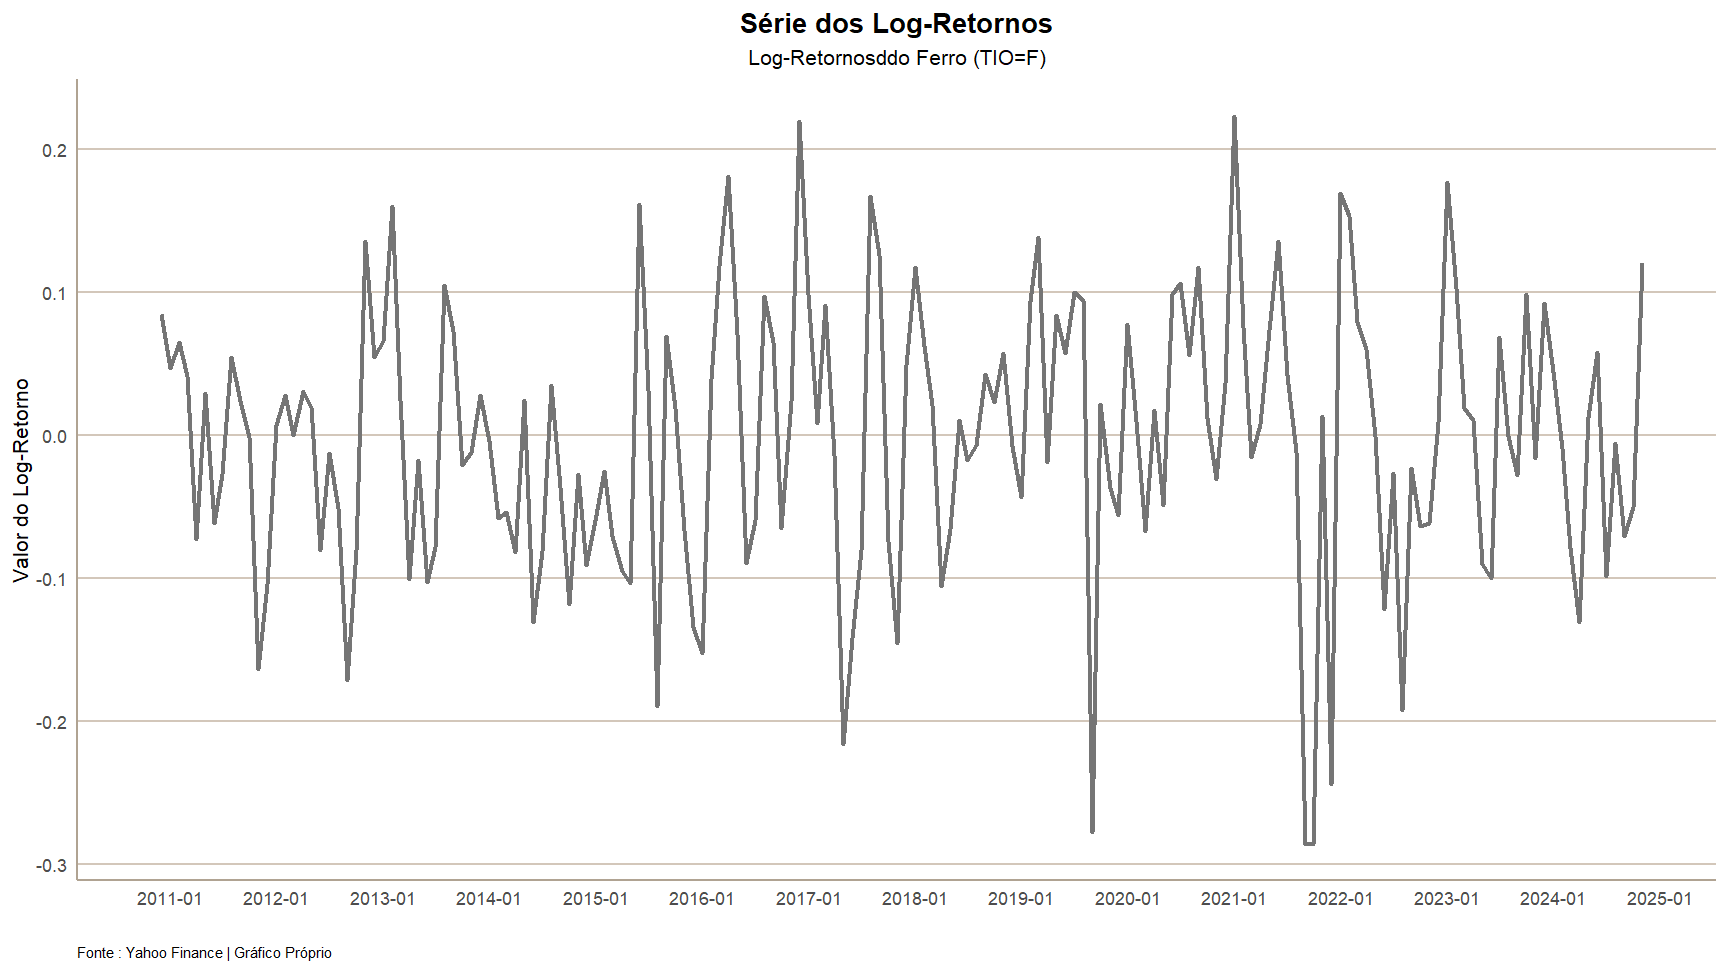
\includegraphics[width=1.0\textwidth]{APS 2/i1qG.png}
    \label{fig:i1qG}
    
    \footnotesize{Fonte: Elaborado pelos autores.}
    \end{figure}

\begin{figure}[H]
    \centering
    \caption{Gráfico de Autocorrelação e Autocorrelação Parcial do Log-Retorno do Ferro (TIO=F)} 
    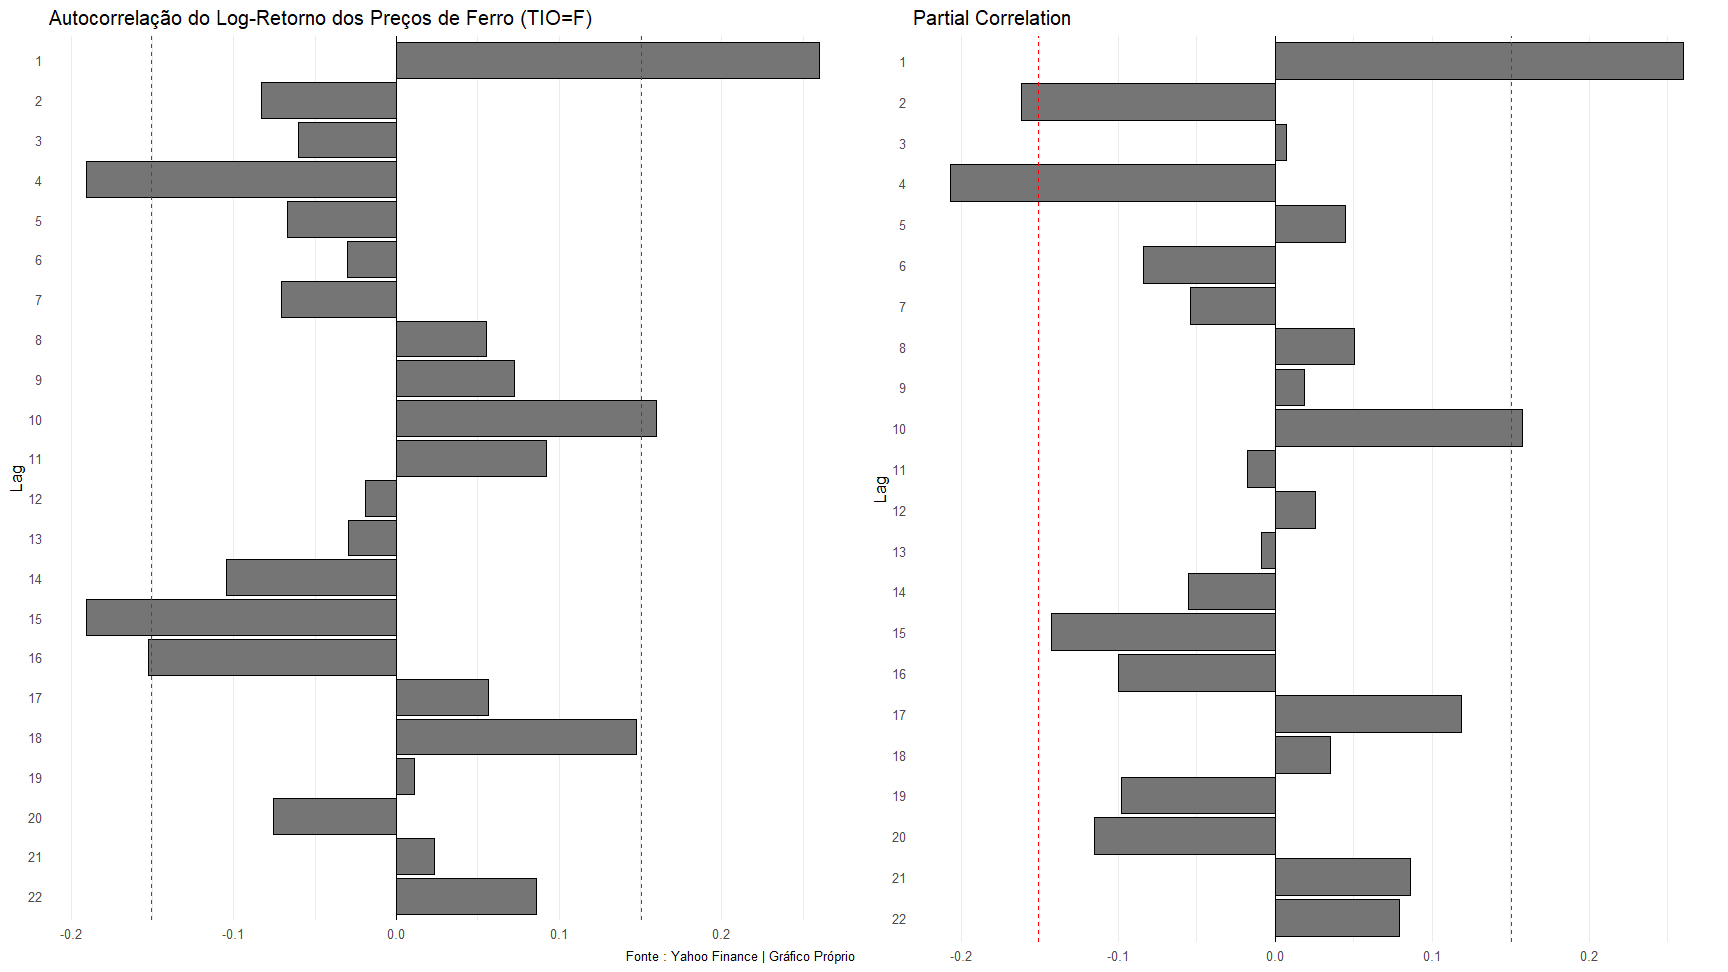
\includegraphics[width=1.0\textwidth]{APS 2/i2qG.png}
    \label{fig:i2qG}
    
    \footnotesize{Fonte: Elaborado pelos autores.}
    \end{figure}

Ao analisar o gráfico de linha da série mensal dos log - retornos do ferro (figura \ref{fig:i1qG}), é notável que os valores oscilam ao redor de uma média, com períodos de maior ou menor volatilidade. Esse comportamento é característico de séries financeiras. É possível observar que alguns clusters de volatilidade estão presentes na série, associados a períodos de incerteza econômica e flutuações nos mercados globais, especialmente em momentos em crises ou eventos globais que impactaram o preço do minério de ferro, como a pandemia de COVID-19 em 2020.

Ambos os correlogramas indicam que a série de log-retornos tem memória de curto prazo até o lag 2, o que reflete o comportamento típico de séries financeiras que apresentam clusters de volatilidade. No entanto, o correlograma sugere a ausência de memória de longo prazo, mesmo que em alguns lags, a barra pareça, visualmente, estar fora do intervalo, a interpretação deve ser feita com cautela, uma vez que nos lags mais avançados, o intervalo de confiança pode ser maior.

\section*{\textbf{Questão H}}
\addcontentsline{toc}{section}{Questão H}

\begin{figure}[H]
    \centering
    \caption{Série Mensal dos Log-Retornos da Vale (VALE)} 
    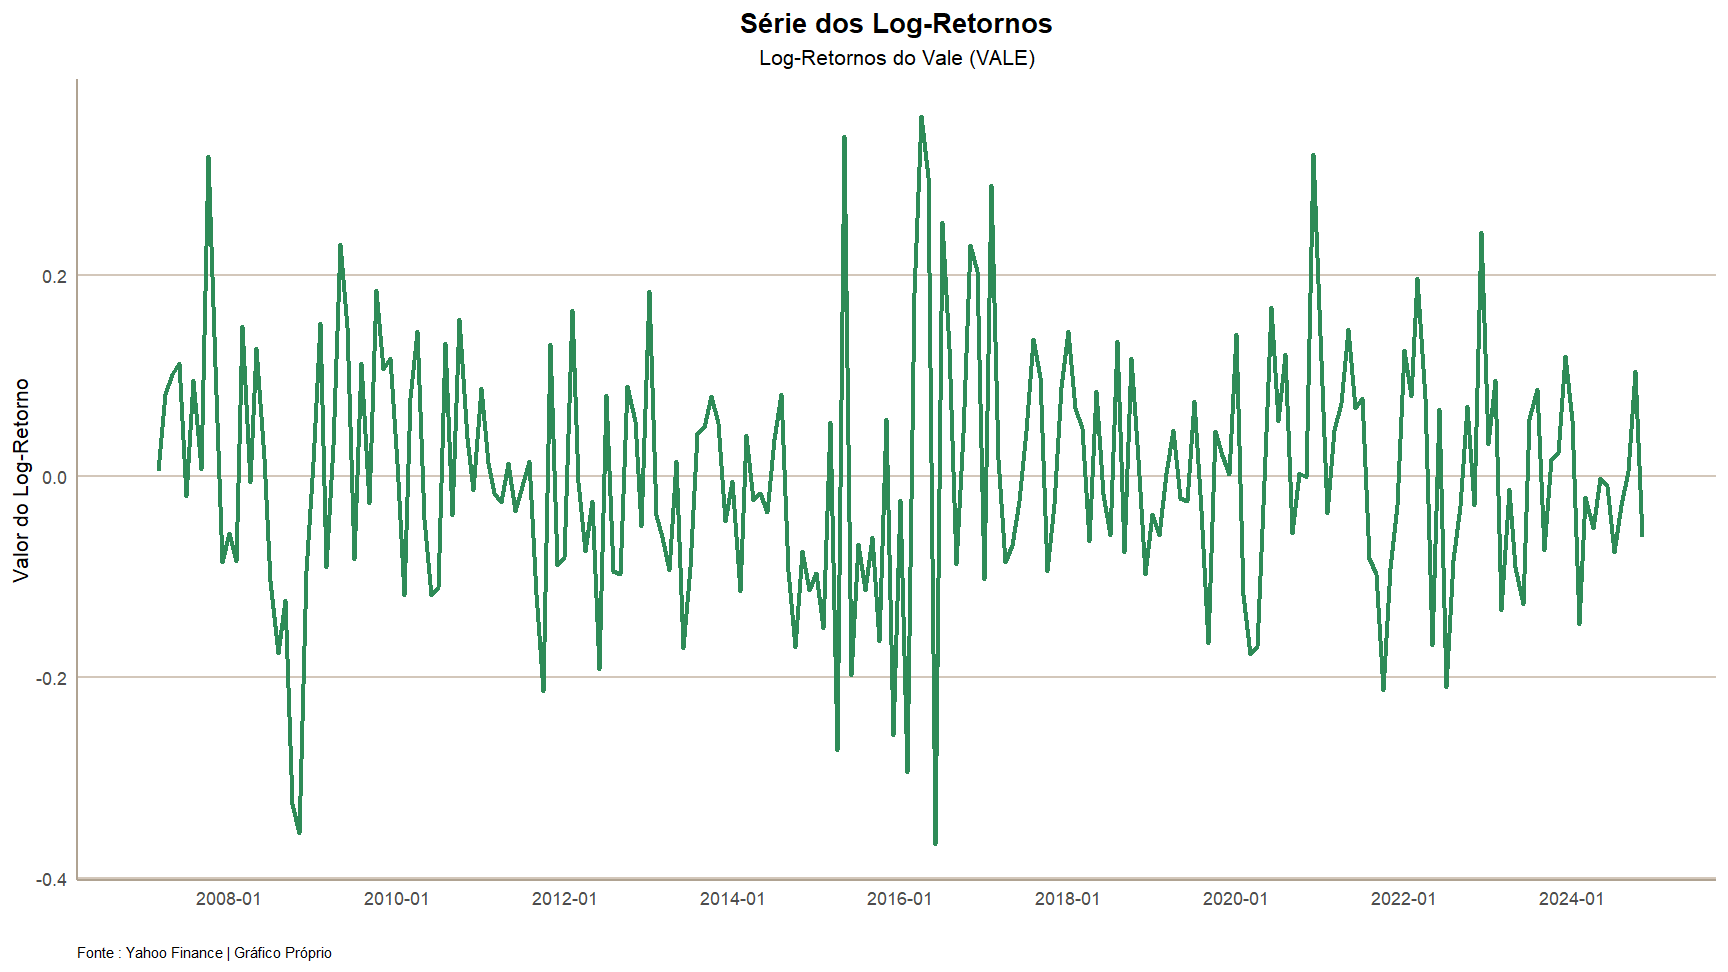
\includegraphics[width=1.0\textwidth]{APS 2/i1qH.png}
    \label{fig:i1qH}
    
    \footnotesize{Fonte: Elaborado pelos autores.}
    \end{figure}

\begin{figure}[H]
    \centering
    \caption{Gráfico de Autocorreção e Autocorreção Parcial do Log-Retorno da Vale (VALE)} 
    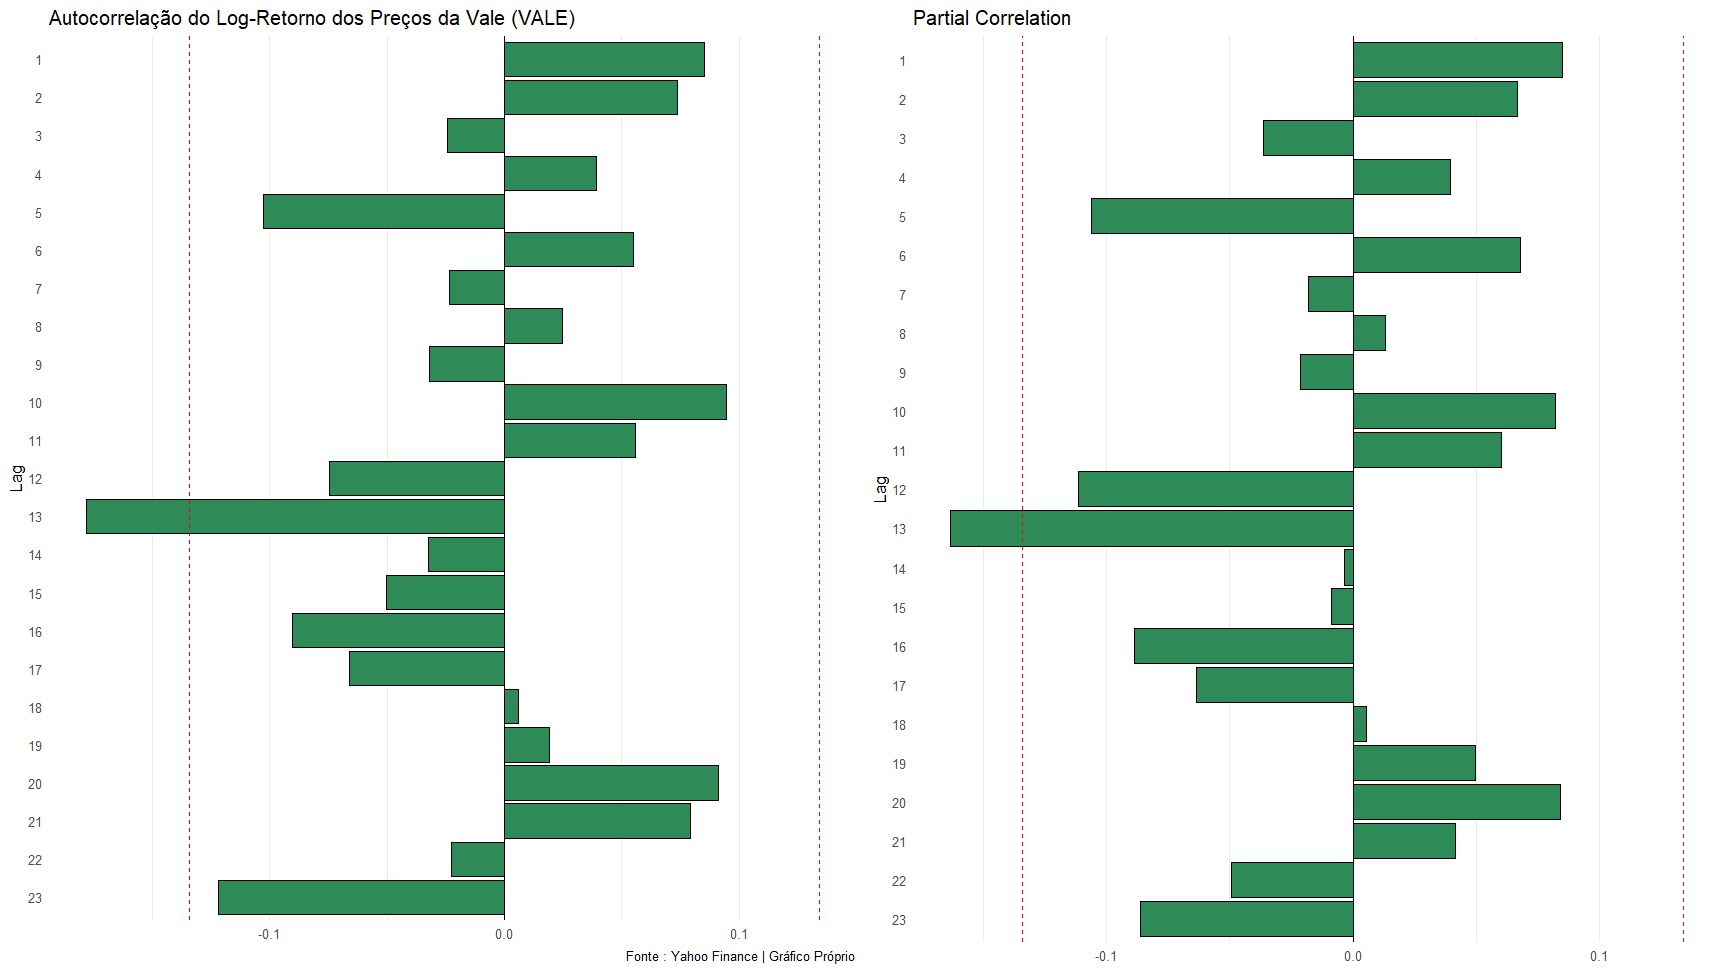
\includegraphics[width=1.0\textwidth]{APS 2/i2qH.png}
    \label{fig:i2qH}
    
    \footnotesize{Fonte: Elaborado pelos autores.}
    \end{figure}

O gráfico de linha da série mensal de log-retornos da Vale evidencia que os retornos oscilam em torno de uma média próxima de zero, o que é característico de uma série estacionária. Isso sugere que, apesar das variações nos retornos, a série retorna uma média constante ao longo do tempo. Assim, como no gráfico de linha anterior para representar a série mensal dos log retornos do ferro (Figura \ref{fig:i1qG}), há evidencias de clusters de volatilidade nessa série. Em 2008-2009, há um aumento da volatilidade, associado à crise financeira global, em 2015 devido à queda dos preços das commodities, especialmente de ferro e em 2020 relacionado à pandemia da COVID-19.

Ao analisar os correlogramas, a presença de autocorrelação significativa nas primeiras defasagens indica que há alguma dependência temporal de curto prazo na série de log-retornos da Vale, o que é esperado em séries de retornos financeiros. Após os primeiros lags, tanto o ACF quanto o PACF mostram que as correlações caem para valores dentro do intervalo de confiança. Isso significa que, em horizontes temporais maiores, a série não exibe dependência dos retornos passados, o que está de acordo com a teoria financeira, que postula que os retornos são independentes e seguem um processo de passeio aleatório (em mercados eficientes). Portanto, a análise dos correlogramas confirma que, embora haja alguma correlação de curto prazo, a série de log-retornos das ações da Vale não possui memória de longo prazo, alinhando-se ao comportamento esperado para séries de retornos financeiros e a série do log-retorno dos preços do minério de ferro.

\section*{\textbf{Questão I}}
\addcontentsline{toc}{section}{Questão I}

De acordo com as teorias de finanças, o preço dos ativos, como o minério de ferro e as ações da Vale, tende a seguir um processo estocástico conhecido como \textbf{passeio aleatório com drift} (o drift é necessário, conforme sustentado pela teoria financeira, visto que os ativos possuem um preço inicial maior que zero), conforme previsto pela \textbf{hipótese de eficiência de mercado}. Essa hipótese sugere que os preços refletem todas as informações disponíveis, tornando seus movimentos futuros imprevisíveis. O passeio aleatório é um processo autorregressivo não estacionário descrito pela equação:

\[
p_t = p_0 + \phi_1 p_{t-1} + a_t \quad ; \quad a_t \sim RB(0, \sigma_a^2)
\]

onde \(\phi_1 = 1\)(coeficiente autorregressivo), caracterizando a presença de uma raiz unitária.

Nos itens \textbf{E} e \textbf{F}, as evidências indicam a presença de raiz unitária, sugerindo que os preços dos ativos seguem um passeio aleatório. Além disso, nos itens \textbf{G} e \textbf{H}, ao analisarmos o correlograma dos log-retornos dos ativos, observamos que a maioria das barras das funções de autocorrelação (FAC) e de autocorrelação parcial (FACP) permaneceu dentro do intervalo de confiança de 95\%. Isso sugere que os log-retornos não apresentam autocorrelações significativas, o que é consistente com um comportamento imprevisível dos ativos.

Portanto, as evidências fornecidas pelos correlogramas dos log-retornos, juntamente com os resultados dos testes de raiz unitária, reforçam a hipótese de que os preços dos ativos são regidos por um processo de passeio aleatório, sem previsibilidade e com comportamento não estacionário.



\section*{\textbf{Questão J}}
\addcontentsline{toc}{section}{Questão J}

A relação de longo prazo mencionada pelo Sr. Tessari entre o preço das ações da Vale e o preço do minério de ferro remete ao conceito de \textbf{cointegração}, conforme discutido em Econometria de Séries Temporais. Como destacado no material de apoio, a cointegração refere-se à existência de um equilíbrio de longo prazo entre duas ou mais séries temporais, mesmo que essas séries individualmente sejam não estacionárias, ou seja, integradas de ordem 1, \(I(1)\).

Para determinar se o preço das ações da Vale e o preço do minério de ferro são cointegrados, devemos seguir alguns passos. Primeiro, realizamos o \textbf{teste de raiz unitária} para verificar se ambas as séries são \(I(1)\). Isso é feito utilizando testes como o \textit{Augmented Dickey-Fuller (ADF)}. Caso ambas as séries apresentem raiz unitária (e amabas apresentam), prosseguimos para a próxima etapa.

Em seguida, estimamos uma \textbf{regressão de cointegração}, na forma \(y_t = \beta_0 + \beta_1 x_t + a_t\), onde \(y_t\) representa o preço das ações da Vale e \(x_t\) o preço do minério de ferro. O resíduo \(a_t\) resultante desta regressão representa os desvios temporários do equilíbrio de longo prazo entre as duas séries.

Por fim, aplicamos o \textbf{teste de raiz unitária nos resíduos} \(a_t\). Se os resíduos forem estacionários \(I(0)\), ou seja, se o teste rejeitar a hipótese nula de presença de raiz unitária, concluímos que as duas séries são cointegradas. Isso indica a existência de uma relação estável de longo prazo, como sugerido na conversa de Tessari.

O conceito de cointegração é fundamental para evitar regressões espúrias, que podem ocorrer ao modelar séries temporais não estacionárias. Além disso, quando as séries são cointegradas, podemos utilizar um \textbf{Modelo de Correção de Erros (MCE)}, como discutido no material de apoio, para modelar os ajustes de curto prazo em direção ao equilíbrio de longo prazo, capturando a dinâmica entre as variáveis de forma mais precisa.

\section*{\textbf{Questão K}}
\addcontentsline{toc}{section}{Questão K}

Para verificar se as séries mensais do preço do minério de ferro e do preço das ações da Vale apresentam uma relação de equilíbrio de longo prazo, aplicamos o \textbf{teste de cointegração de Engle-Granger}. Como ambas as séries possuem raiz unitária, conduzimos uma regressão de cointegração entre as duas séries.

Após estimar a regressão, aplicamos o \textit{teste ADF} nos resíduos para verificar se possuem raiz unitária. Se os resíduos forem \(I(0)\), isso indicaria que as séries são cointegradas, ou seja, existe uma relação de equilíbrio de longo prazo entre o preço do minério de ferro e o preço das ações da Vale.

\section*{\textbf{Questão L \& M}}
\addcontentsline{toc}{section}{Questão L \& M}

\begin{equation}
    y_t=\beta_0+\beta_1x_t+\epsilon_t
    \label{eq:ml}
\end{equation}

\begin{table}[H]
\centering
\caption{Resultados da Regressão Linear do Modelo}
\renewcommand{\arraystretch}{0.9} % Reduz o espaçamento entre as linhas
\resizebox{0.9\textwidth}{!}{ % Reduz a largura da tabela para 90% da largura do texto
    \footnotesize % Usa uma fonte menor
    \begin{tabular}{@{\extracolsep{5pt}}lccc} 
    \\[-1.8ex]\hline 
    \hline \\[-1.8ex] 
    & Estimativa & Erro Padrão & Valor t \\ 
    \hline \\[-1.8ex]  
    $\beta_0$\textbf{(Intercepto)}  & -3.2047  & 0.2646  & -12.11 *** \\ 
    $\beta_1$($x_t$)      & 1.1471   & 0.0572  & 20.05 *** \\ 
    \hline \\[-1.8ex] 
    Erro padrão residual & \multicolumn{3}{c}{0.2783 \textit{(df = 167)}} \\ 
    R-quadrado múltiplo  & \multicolumn{3}{c}{0.7066} \\ 
    R-quadrado ajustado  & \multicolumn{3}{c}{0.7048} \\ 
    Estatística F        & \multicolumn{3}{c}{402.2 \textit{(df = 1, 167)}, p-valor: < 2.2e-16} \\ 
    \hline 
    \end{tabular}
}
\label{tab:ml_summary}
\end{table}

\begin{equation}
    \Delta \epsilon_t = \gamma  \epsilon_{t-1} + \delta \Delta  \epsilon_{t-1} + a_t \ \ ; \ \ a_t \sim RB(0, \sigma_a^2)   
    \label{eq:talml}
\end{equation}

\begin{table}[H] 
\centering 
  \caption{Resultados do Teste ADF Apenas com Defasagens do Resíduo da Equação \ref{eq:talml}} 
  \renewcommand{\arraystretch}{0.9} % Reduz o espaçamento entre as linhas
  \resizebox{0.9\textwidth}{!}{ % Reduz a largura da tabela para 90% da largura do texto
    \footnotesize % Usa uma fonte menor
  \begin{tabular}{@{\extracolsep{5pt}}lccc} 
  \\[-1.8ex]\hline 
  \hline \\[-1.8ex] 
  & Estimate & Std. Error & t value \\ 
  \hline \\[-1.8ex] 
  $\gamma$ (\textbf{Coef UR})  & $-0.07485$ & $0.03560$ & $-2.103^{*}$ \\ 
  $\delta$ (\textbf{Coef Lag}) & $-0.25010$ & $0.07822$ & $-3.197^{**}$ \\ 
  \hline \\[-1.8ex] 
  Erro padrão residual & \multicolumn{3}{c}{$0.1237$ \textit{(df = 156)}} \\ 
  R-quadrado múltiplo & \multicolumn{3}{c}{$0.109$} \\ 
  R-quadrado ajustado & \multicolumn{3}{c}{$0.09759$} \\ 
  Estatística-F & \multicolumn{3}{c}{$9.543$ \textit{(df = 2; 156)}, p-value: $0.0001231$} \\ 
  Valor do Teste & \multicolumn{3}{c}{$-2.1027$} \\ 
  \hline 
  \textbf{Valores Críticos para o Teste de Cointegração (Engle-Granger)} & \multicolumn{3}{c}{} \\ 
  \hline
  & 1\% & 5\% & 10\% \\ 
  T = 50 & -4.123 & -3.461 & -3.130 \\ 
  T = 100 & -4.008 & -3.398 & -3.087 \\ 
  T = 200 & -3.954 & -3.368 & -3.067 \\ 
  T = 500 & -3.921 & -3.350 & -3.054 \\ 
  \hline 
  \hline \\[-1.8ex] 
  \textit{Note:} & \multicolumn{3}{r}{$^{***}$Significant at 0.1\% level} \\ 
  \end{tabular} 
 }
 \label{tab:adfml}
\end{table}


\begin{equation}
    \Delta y_t=\alpha_0+\alpha_1 \Delta x_t+u_t
    \label{eq:mdl}
\end{equation}

\begin{table}[H]
\centering
\caption{Resultados da Regressão Linear do Modelo na Diferença}
\renewcommand{\arraystretch}{0.9} % Reduz o espaçamento entre as linhas
\resizebox{0.9\textwidth}{!}{ % Reduz a largura da tabela para 90% da largura do texto
    \footnotesize % Usa uma fonte menor
    \begin{tabular}{@{\extracolsep{5pt}}lccc} 
    \\[-1.8ex]\hline 
    \hline \\[-1.8ex] 
    & Estimativa & Erro Padrão & Valor t \\ 
    \hline \\[-1.8ex]  
    $\alpha_0$\textbf{(Intercepto)}  & -0.0006  & 0.0086  & -0.073 \\ 
    $\alpha_1$($\Delta x_t$)   & 0.4936   & 0.0907  & 5.44 *** \\ 
    \hline \\[-1.8ex] 
    Erro padrão residual & \multicolumn{3}{c}{0.1119 \textit{(df = 166)}} \\ 
    R-quadrado múltiplo  & \multicolumn{3}{c}{0.1514} \\ 
    R-quadrado ajustado  & \multicolumn{3}{c}{0.1463} \\ 
    Estatística F        & \multicolumn{3}{c}{29.62 \textit{(df = 1, 166)}, p-valor: 1.859e-07} \\ 
    \hline 
    \end{tabular}
}
\label{tab:mdl_summary}
\end{table}

\begin{equation}
    \Delta u_t = \gamma  u_{t-1} + \delta \Delta u_{t-1} + a_t \ \ ; \ \ a_t \sim RB(0, \sigma_a^2)   
    \label{eq:talmdl}
\end{equation}


\begin{table}[H] 
\centering 
  \caption{Resultados do Teste ADF Apenas com Defasagens do Resíduo da Equação \ref{eq:talmdl}} 
  \renewcommand{\arraystretch}{0.9} % Reduz o espaçamento entre as linhas
  \resizebox{0.9\textwidth}{!}{ % Reduz a largura da tabela para 90% da largura do texto
    \footnotesize % Usa uma fonte menor
  \begin{tabular}{@{\extracolsep{5pt}}lccc} 
  \\[-1.8ex]\hline 
  \hline \\[-1.8ex] 
  & Estimate & Std. Error & t value \\ 
  \hline \\[-1.8ex] 
  $\gamma$ (\textbf{Coef UR})  & $-1.29000$ & $0.12376$ & $-10.42^{***}$ \\ 
  $\delta$ (\textbf{Coef Lag}) & $0.03957$ & $0.07921$ & $0.50$ \\ 
  \hline \\[-1.8ex] 
  Erro padrão residual & \multicolumn{3}{c}{$0.1103$ \textit{(df = 155)}} \\ 
  R-quadrado múltiplo & \multicolumn{3}{c}{$0.6253$} \\ 
  R-quadrado ajustado & \multicolumn{3}{c}{$0.6204$} \\ 
  Estatística-F & \multicolumn{3}{c}{$129.3$ \textit{(df = 2; 155)}, p-value: $< 2.2e-16$} \\ 
  Valor do Teste & \multicolumn{3}{c}{$-10.4238$} \\ 
  \hline 
  \textbf{Valores Críticos para o Teste de Cointegração (Engle-Granger)} & \multicolumn{3}{c}{} \\ 
  \hline
  & 1\% & 5\% & 10\% \\ 
  T = 50 & -4.123 & -3.461 & -3.130 \\ 
  T = 100 & -4.008 & -3.398 & -3.087 \\ 
  T = 200 & -3.954 & -3.368 & -3.067 \\ 
  T = 500 & -3.921 & -3.350 & -3.054 \\ 
  \hline 
  \hline \\[-1.8ex] 
  \textit{Note:} & \multicolumn{3}{r}{$^{***}$Significant at 0.1\% level} \\ 
  \end{tabular} 
 }
 \label{tab:adfmdl}
\end{table}

Com base nas análises realizadas até o momento, nossa equipe propõe o uso de um \textbf{Modelo de Correção de Erros (MCE)} em vez de um modelo de regressão linear simples ou nas primeiras diferenças. Essa recomendação baseia-se nos resultados encontrados e no conceito de cointegração.

Primeiramente, ao observar os resultados da regressão linear original (\ref{eq:ml}), o coeficiente $\beta_1$ estimado em 1.1471 mostrou-se altamente significativo, conforme visto na Tabela \ref{tab:ml_summary}. Isso indica uma forte relação entre $x_t$ e $y_t$. No entanto, como estamos trabalhando com séries temporais, é necessário verificar a estacionariedade para evitar regressões espúrias, o que não é garantido apenas pela significância dos coeficientes.

Com base nessa preocupação, realizamos o teste de Dickey-Fuller Aumentado (ADF) sobre os resíduos da equação (\ref{eq:talml}). O coeficiente $\gamma$, estimado em -0.07485, foi significativo ao nível de 5\% (Tabela \ref{tab:adfml}), indicando que os resíduos possuem raiz unitária. O valor do teste ADF foi de -2.1027, o que, comparado aos valores críticos, sugere que não podemos rejeitar a hipótese nula de raiz unitária nesse nível de significância. Esse resultado reforça a ideia de que as séries podem ser cointegradas, ou seja, possuem uma relação de equilíbrio de longo prazo.

Em seguida, ao modelar as variáveis nas primeiras diferenças, conforme a equação \ref{eq:mdl}, encontramos que o coeficiente $\alpha_1$ estimado em 0.4936 foi estatisticamente significativo (Tabela \ref{tab:mdl_summary}). Isso sugere que, no curto prazo, as variações de $x_t$ impactam de maneira significativa as variações de $y_t$. No entanto, essa abordagem nas primeiras diferenças pode não capturar adequadamente a relação de longo prazo entre as séries, já que ela se concentra apenas nas mudanças instantâneas, ignorando possíveis correções de equilíbrio.

Por fim, o teste ADF nos resíduos do modelo de diferenças (\ref{eq:talmdl}) apresentou um valor altamente significativo para o coeficiente $\gamma$ (-1.29000) (Tabela \ref{tab:adfmdl}), o que rejeita a hipótese de raiz unitária e confirma que os resíduos são estacionários. Isso sugere a presença de cointegração entre as séries $y_t$ e $x_t$.

Diante desses resultados, propomos o uso de um \textbf{Modelo de Correção de Erros (MCE)}, que combina a dinâmica de curto prazo com a relação de longo prazo, capturando tanto as variações imediatas quanto os desvios do equilíbrio. A equação do modelo é:

\begin{equation}
    \Delta y_t = \alpha_0 + \alpha_1 \Delta x_t + \gamma u_{t-1} + \epsilon_t
\end{equation}

Nesse modelo, $\alpha_1$ captura a relação de curto prazo entre as variações de $x_t$ e $y_t$, enquanto $\gamma u_{t-1}$ representa o termo de correção de erros, ajustando os desvios em relação ao equilíbrio de longo prazo. O coeficiente $\gamma$ indica a velocidade com que os desvios são corrigidos ao longo do tempo, sendo negativo e significativo, conforme esperado.

Portanto, nossa equipe conclui que o MCE é a escolha mais adequada, uma vez que reflete tanto a dinâmica de curto prazo quanto a relação de longo prazo entre $y_t$ e $x_t$, fornecendo uma modelagem mais completa das variáveis.


\section*{\textbf{Questão N}}
\addcontentsline{toc}{section}{Questão N}

O preço do minério de ferro tem apresentado volatilidade significativa recentemente, influenciado por diversos fatores econômicos e geopolíticos.

\textbf{Perspectiva Atual do Preço do Minério de Ferro:} Atualmente, os preços futuros do minério de ferro na China têm registrado quedas, atribuídas a uma oferta global mais robusta e a uma demanda doméstica mais fraca. Além disso, as expectativas de estímulos fiscais adicionais por parte do governo chinês têm impactado o mercado, embora de forma limitada.

\textbf{Fatores que Influenciaram a Dinâmica Recente do Preço:}
\begin{itemize}
    \item \textit{Demanda Chinesa:} A China, maior consumidora mundial de minério de ferro, tem apresentado uma demanda reduzida, influenciada por dados econômicos mistos e restrições ambientais que afetam a produção de aço.
    
    \item \textit{Oferta Global:} O aumento na produção global, especialmente por parte de grandes mineradoras, elevou a oferta disponível no mercado, pressionando os preços para baixo.
    
    \item \textit{Políticas Econômicas:} As incertezas relacionadas a possíveis estímulos econômicos na China e políticas comerciais internacionais têm criado volatilidade nos preços, com investidores reagindo a anúncios e especulações sobre medidas governamentais.
\end{itemize}

\textbf{Recomendação sobre as Ações da Vale:} Considerando o cenário atual, analistas têm diferentes perspectivas sobre as ações da Vale (VALE). Alguns destacam que, apesar da queda nos preços do minério de ferro, a Vale mantém uma produção sólida e iniciativas estratégicas, como investimentos em sustentabilidade e inovação tecnológica. Outros apontam que a volatilidade do mercado e a dependência da demanda chinesa são fatores de risco a serem considerados.

Portanto, é essencial que investidores avaliem seu perfil de risco e consultem fontes especializadas antes de tomar decisões de investimento.

\newpage
\begin{thebibliography}{}

\bibitem{wickham2015ggplot2}
WICKHAM, Hadley; SIEVERT, Carson. \textit{ggplot2: Elegant Graphics for Data Analysis}. 2. ed. New York: Springer, 2015.

\bibitem{wickham2023rds}
WICKHAM, Hadley; ÇETINKAYA-RUNDEL, Mine; GROLEMUND, Garrett. \textit{R for Data Science: Import, Tidy, Transform, Visualize, and Model Data}. 2. ed. Sebastopol: O'Reilly Media, 2023.

\bibitem{scheuch2023tidy}
SCHEUCH, Christoph; VOIGT, Stefan; WEISS, Patrick. \textit{Tidy Finance with R}. 1. ed. Boca Raton: CRC Press, 2023.

\bibitem{heiss2020intro}
HEISS, Florian. \textit{Using R for Introductory Econometrics}. 2. ed. Düsseldorf: Florian Heiss, 2020. Disponível em: \url{http://www.URfIE.net}.

\bibitem{pfaff2024urca}
PFAFF, Bernhard; ZIVOT, Eric; STIGLER, Matthieu. \textit{urca: Unit Root and Cointegration Tests for Time Series Data}. R package version 1.3-4, 2024. Disponível em: \url{https://cran.r-project.org/web/packages/urca/}.

\end{thebibliography}


\end{document}
